\documentclass[11pt,a4paper]{article}
\usepackage[T1]{fontenc}
\usepackage[utf8]{inputenc}
\usepackage{lmodern}
\usepackage{amsmath,amssymb}
\usepackage{graphicx}
\usepackage{booktabs}
\usepackage{array}
\usepackage{longtable}
\usepackage{xcolor}
\usepackage[hidelinks]{hyperref}

% A4 with 2.5-cm margins (set by hand: only packages that ship with every installation are used)
\setlength{\textwidth}{160mm}\setlength{\oddsidemargin}{25mm}\addtolength{\oddsidemargin}{-1in}
\setlength{\evensidemargin}{\oddsidemargin}
\setlength{\topmargin}{20mm}\addtolength{\topmargin}{-1in}\setlength{\headheight}{0pt}\setlength{\headsep}{0pt}
\setlength{\textheight}{247mm}\setlength{\footskip}{10mm}
\setlength{\parindent}{0pt}\setlength{\parskip}{5pt plus 1pt}
\setlength{\emergencystretch}{1.5em}
\renewcommand{\thesection}{S\arabic{section}}
\renewcommand{\thetable}{S\arabic{table}}
\renewcommand{\thefigure}{S\arabic{figure}}
\setlength{\LTcapwidth}{\textwidth}
\setlength{\abovecaptionskip}{4pt}
% Figures float as in the article (D108): at most two per page with text between them, a page of their own only
% when they fill most of it; tables stay where they are written
\setcounter{topnumber}{1}\setcounter{bottomnumber}{1}\setcounter{totalnumber}{2}
\renewcommand{\topfraction}{0.85}\renewcommand{\bottomfraction}{0.6}\renewcommand{\textfraction}{0.1}
\renewcommand{\floatpagefraction}{0.8}
\makeatletter\setlength{\@fpsep}{\textheight}\makeatother

% Tables and figures are placed where they are written (no floats), each kept on one page with its caption
\makeatletter
\newenvironment{stable}{\par\addvspace{8pt}\noindent\begin{minipage}{\textwidth}\def\@captype{table}\centering}{\end{minipage}\par\addvspace{8pt}}
\newenvironment{sfigure}{\par\addvspace{8pt}\noindent\begin{minipage}{\textwidth}\def\@captype{figure}\centering}{\end{minipage}\par\addvspace{8pt}}
\makeatother

\begin{document}

\begin{center}
{\Large\bfseries Supplementary material}\\[6pt]
{\large Grid event or data artefact? Hierarchical weak supervision for anomaly attribution in multi-city feeder telemetry}\\[8pt]
Saad Farah, Lahcen Hassine, Hatim Lechgar, Anass Rghioui
\end{center}

This supplement gives the evidence behind statements of the article that its main tables and figures do not show: the
real-data events and clock days (Section~\ref{sec:s-real}), the rules and the label model (Section~\ref{sec:s-rules}),
the detector and the end model on the real data (Section~\ref{sec:s-detector}), the full injection benchmark
(Section~\ref{sec:s-benchmark}), the downstream test (Section~\ref{sec:s-downstream}), the transfer test
(Section~\ref{sec:s-transfer}), and the software versions, settings, run times and seeds (Section~\ref{sec:s-repro}).
Every number is read from the result files released with the code at \url{https://github.com/farah1902/grid-event-or-data-artefact-code}, where the typed catalogue
(404 entries) is also released as a CSV file.

Conventions. Time stamps are as recorded. Zones: L1--L5 La\^ayoune, B1--B3 Boujdour, F1--F7 Foum El Oued, M1--M2 Marrakech.
Types: A1 zero-fill gap, A2 simultaneous fill, A3 single-zone fill, A4 clock error, G1 regional outage, G2 city outage,
G3 unplanned feeder outage, G4 planned work, G5 load transfer, N normal or untyped. Unless stated otherwise, results on
injected data are for the test period (July 2023 -- May 2024) and are means $\pm$ s.d.\ over the 10 test seeds of each
contamination rate (1, 3 and 7\%); $p$-values are from exact paired two-sided Wilcoxon signed-rank tests, whose smallest
attainable value over 10 seeds is 0.002. Untuned event formation means $(w, q, g_{\max}) = (1, 99.5\%, 1)$.

\tableofcontents

\clearpage\section{Real-data events and clock days}\label{sec:s-real}
\begin{stable}
\caption{Key events on the real data. Each row is a rule item with its final label and confidence; rows between two horizontal lines form one episode, whose items' labels are listed in time order with their confidence. Times as recorded. The January 2023 episode is shown in Fig.~4 of the article, the episode of 31 March -- 2 April 2024 in Fig.~5 and the episode of 16 July 2023 in Fig.~\ref{fig:s-jul2023}.}\label{tab:s-key-events}
\scriptsize\setlength{\tabcolsep}{3.5pt}
\begin{tabular}{@{}l r l l c c >{\raggedright\arraybackslash}p{4.3cm}@{}}
\toprule
Start & Duration (h) & Zones & Item & Label & Conf. & Episode: labels in time order \\
\midrule
2022-09-26 08:20 & 0.83 & L1--L5 & dead & G2 & 0.99 & G2(0.99) \\
\midrule
2022-10-23 08:10 & 1.50 & L5 & dead & G4 & 0.96 & G4(0.96) $\rightarrow$ A3(1.00) $\rightarrow$ A3(1.00) $\rightarrow$ G3(0.70) \\
2022-10-23 09:40 & 1.50 & L5 & fill & A3 & 1.00 & G4(0.96) $\rightarrow$ A3(1.00) $\rightarrow$ A3(1.00) $\rightarrow$ G3(0.70) \\
2022-10-23 11:20 & 7.17 & L5 & fill & A3 & 1.00 & G4(0.96) $\rightarrow$ A3(1.00) $\rightarrow$ A3(1.00) $\rightarrow$ G3(0.70) \\
2022-10-23 18:30 & 15.00 & L5 & dead & G3 & 0.70 & G4(0.96) $\rightarrow$ A3(1.00) $\rightarrow$ A3(1.00) $\rightarrow$ G3(0.70) \\
\midrule
2022-10-29 20:40 & 108.17 & F4 & dead & G3 & 0.97 & G3(0.97) $\rightarrow$ A3(1.00) \\
2022-11-03 08:50 & 1.67 & F4 & fill & A3 & 1.00 & G3(0.97) $\rightarrow$ A3(1.00) \\
\midrule
2022-11-16 22:40 & 10.17 & F1 & dead & G3 & 0.83 & G3(0.83) $\rightarrow$ A3(1.00) \\
2022-11-17 08:50 & 2.00 & F1 & fill & A3 & 1.00 & G3(0.83) $\rightarrow$ A3(1.00) \\
\midrule
2023-01-26 01:20 & 36.00 & L1--L5 & fill & A2 & 1.00 & A2(1.00) $\rightarrow$ A2(1.00) $\rightarrow$ A1(0.99) \\
2023-01-26 02:10 & 67.00 & B1--B3, F1--F7 & fill & A2 & 1.00 & A2(1.00) $\rightarrow$ A2(1.00) $\rightarrow$ A1(0.99) \\
2023-01-28 21:10 & 13.67 & all 15 southern zones & dead & A1 & 0.99 & A2(1.00) $\rightarrow$ A2(1.00) $\rightarrow$ A1(0.99) \\
\midrule
2023-02-10 08:20 & 42.33 & F6 & dead & G3 & 0.84 & G3(0.84) $\rightarrow$ A3(1.00) \\
2023-02-12 02:40 & 12.17 & F6 & fill & A3 & 1.00 & G3(0.84) $\rightarrow$ A3(1.00) \\
\midrule
2023-07-16 14:50 & 16.17 & B1--B3, F1--F7 & dead & A1 & 0.93 & A1(0.93) $\rightarrow$ A2(1.00) \\
2023-07-16 15:30 & 15.50 & L1--L5 & fill & A2 & 1.00 & A1(0.93) $\rightarrow$ A2(1.00) \\
\midrule
2024-03-31 09:10 & 2.00 & B1--B3, F1--F7 & fill & A2 & 1.00 & A2(1.00) $\rightarrow$ A1(1.00) $\rightarrow$ A2(0.99) $\rightarrow$ G4(0.89) \\
2024-03-31 11:10 & 43.83 & B1--B3, F1--F7, L3--L5 & dead & A1 & 1.00 & A2(1.00) $\rightarrow$ A1(1.00) $\rightarrow$ A2(0.99) $\rightarrow$ G4(0.89) \\
2024-03-31 11:10 & 43.00 & L1, L2 & fill & A2 & 0.99 & A2(1.00) $\rightarrow$ A1(1.00) $\rightarrow$ A2(0.99) $\rightarrow$ G4(0.89) \\
2024-04-02 06:10 & 0.83 & L1 & dead & G4 & 0.89 & A2(1.00) $\rightarrow$ A1(1.00) $\rightarrow$ A2(0.99) $\rightarrow$ G4(0.89) \\
\bottomrule
\end{tabular}
\end{stable}

\begin{sfigure}
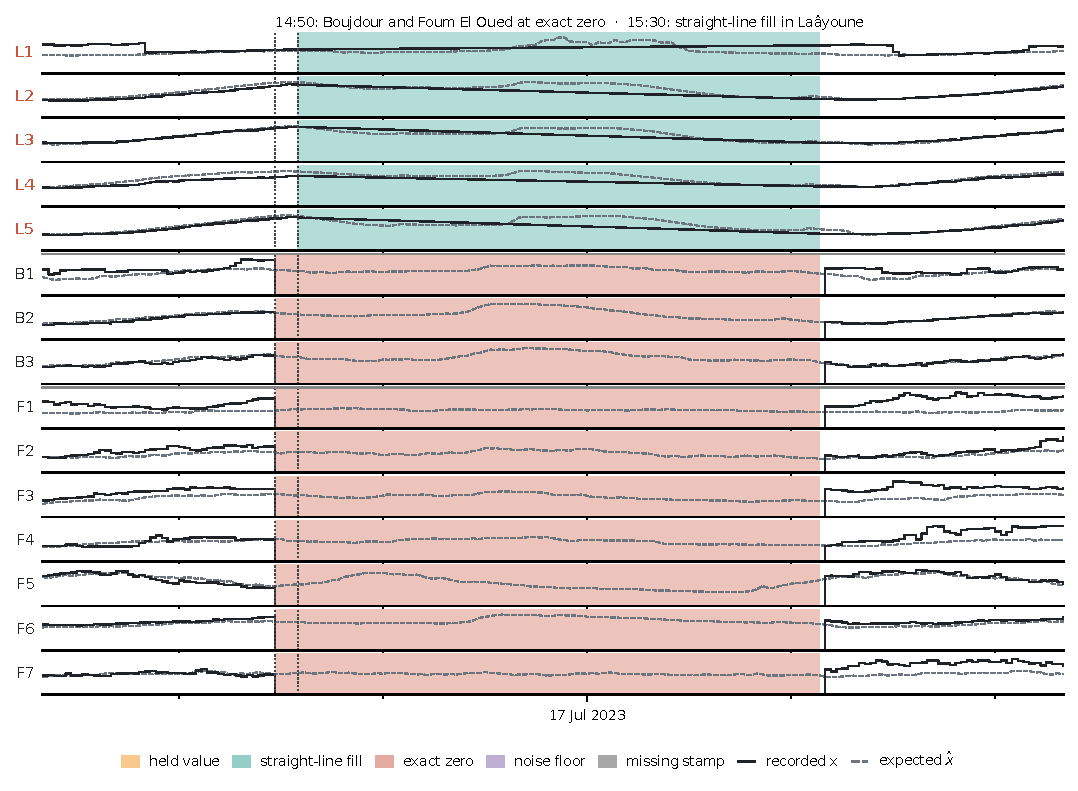
\includegraphics[width=\textwidth]{figures/FigS1}
\caption{The only regional-outage candidate, 16--17 July 2023 (time stamps as recorded). Boujdour and Foum El Oued read exact zeros from 14:50 for 16.2~h (A1, confidence 0.93) while every Laâyoune zone is filled by straight lines from 15:30 for 15.5~h (A2, 1.00): a recording failure, not an outage. Shading: per-step states; dashed line: expected value; dotted lines: the two start times.}\label{fig:s-jul2023}
\end{sfigure}

\begingroup\scriptsize\setlength{\tabcolsep}{4pt}
\begin{longtable}{@{}l l l r r r r r l@{}}
\caption{Clock days: the rule items of kind clock. Calendar change: the European change of summer time (Europe) or Morocco's suspension of GMT+1 for Ramadan and its return (Morocco); the other Marrakech days have stamp anomalies only. Duplicated stamps and missing steps come from the audit of the recorded time stamps. $\delta^{*}$ is the shift (within $\pm$120~min) that maximises the correlation between the mean daily profiles of the 7 days before and the 7 days after the date (Fig.~\ref{fig:s-clock}); the correlations are those at zero shift and at $\delta^{*}$. Final label of the label model.}\label{tab:s-clock}\\
\toprule
Date & City & Calendar & Duplicated & Missing & $\delta^{*}$ & Corr. & Corr. & Final label \\
 & & change & stamps & steps & (min) & at 0 & at $\delta^{*}$ & (confidence) \\
\midrule
\endfirsthead
\multicolumn{9}{@{}l}{\emph{Table \thetable, continued}}\\
\toprule
Date & City & Calendar & Duplicated & Missing & $\delta^{*}$ & Corr. & Corr. & Final label \\
 & & change & stamps & steps & (min) & at 0 & at $\delta^{*}$ & (confidence) \\
\midrule
\endhead
\bottomrule
\endfoot
2022-10-30 & Laâyoune & Europe & 6 & 0 & -60 & 0.8775 & 0.9845 & A4 (0.98) \\
2023-03-19 & Laâyoune & Morocco & 0 & 0 & +30 & 0.8385 & 0.8448 & N (0.97) \\
2023-03-26 & Laâyoune & Europe & 0 & 0 & +20 & 0.7925 & 0.7986 & N (0.95) \\
2023-04-23 & Laâyoune & Morocco & 0 & 6 & -120 & 0.6932 & 0.7747 & A4 (0.70) \\
2023-10-29 & Laâyoune & Europe & 6 & 0 & -120 & 0.6465 & 0.9972 & A4 (0.98) \\
2024-03-10 & Laâyoune & Morocco & 0 & 0 & +120 & 0.5915 & 0.7119 & N (0.97) \\
2024-03-31 & Laâyoune & Europe & 0 & 0 & 0 & 0.9868 & 0.9868 & N (0.95) \\
2024-04-14 & Laâyoune & Morocco & 0 & 6 & -20 & 0.8558 & 0.8603 & A4 (0.70) \\
\midrule
2022-10-30 & Boujdour & Europe & 6 & 0 & -60 & 0.8802 & 0.9781 & A4 (0.98) \\
2023-03-19 & Boujdour & Morocco & 0 & 0 & 0 & 0.9025 & 0.9025 & N (0.97) \\
2023-03-26 & Boujdour & Europe & 0 & 0 & 0 & 0.9292 & 0.9292 & N (0.95) \\
2023-04-23 & Boujdour & Morocco & 0 & 6 & +20 & 0.8416 & 0.8469 & A4 (0.70) \\
2023-10-29 & Boujdour & Europe & 6 & 0 & -60 & 0.8671 & 0.9809 & A4 (0.98) \\
2024-03-10 & Boujdour & Morocco & 0 & 0 & -120 & 0.6704 & 0.8175 & N (0.97) \\
2024-03-31 & Boujdour & Europe & 0 & 0 & +60 & 0.9027 & 0.9889 & N (0.60) \\
2024-04-14 & Boujdour & Morocco & 0 & 6 & +20 & 0.9125 & 0.9181 & A4 (0.70) \\
\midrule
2022-10-30 & Foum El Oued & Europe & 6 & 0 & -60 & 0.8674 & 0.9362 & A4 (0.98) \\
2023-03-19 & Foum El Oued & Morocco & 0 & 0 & +20 & 0.8805 & 0.8875 & N (0.97) \\
2023-03-26 & Foum El Oued & Europe & 0 & 0 & -90 & 0.6628 & 0.7529 & N (0.95) \\
2023-04-23 & Foum El Oued & Morocco & 0 & 6 & -60 & 0.8614 & 0.9096 & A4 (0.70) \\
2023-10-29 & Foum El Oued & Europe & 6 & 0 & -60 & 0.7486 & 0.8509 & A4 (0.83) \\
2024-03-10 & Foum El Oued & Morocco & 0 & 0 & -60 & 0.7827 & 0.8531 & N (0.97) \\
2024-03-31 & Foum El Oued & Europe & 0 & 0 & +60 & 0.5843 & 0.7667 & N (0.95) \\
2024-04-14 & Foum El Oued & Morocco & 0 & 6 & -120 & 0.6929 & 0.8425 & A4 (0.70) \\
\midrule
2023-01-09 & Marrakech & -- & 0 & 19 & -- & -- & -- & N (0.95) \\
2023-03-19 & Marrakech & Morocco & 0 & 0 & +30 & 0.9444 & 0.9610 & N (0.97) \\
2023-03-26 & Marrakech & Europe & 0 & 0 & -30 & 0.9102 & 0.9387 & N (0.95) \\
2023-04-10 & Marrakech & -- & 0 & 2 & -90 & 0.0928 & 0.2779 & N (0.97) \\
2023-04-11 & Marrakech & -- & 2 & 0 & -90 & 0.0742 & 0.2966 & A4 (0.83) \\
2023-04-23 & Marrakech & Morocco & 0 & 0 & 0 & 0.6976 & 0.6976 & N (0.95) \\
2023-08-16 & Marrakech & -- & 0 & 1 & +120 & 0.6610 & 0.7916 & N (0.97) \\
2023-08-23 & Marrakech & -- & 1 & 3 & -30 & 0.9238 & 0.9449 & A4 (0.83) \\
2023-10-29 & Marrakech & Europe & 0 & 0 & -30 & 0.7483 & 0.7886 & N (0.97) \\
\end{longtable}
\endgroup

\begin{sfigure}
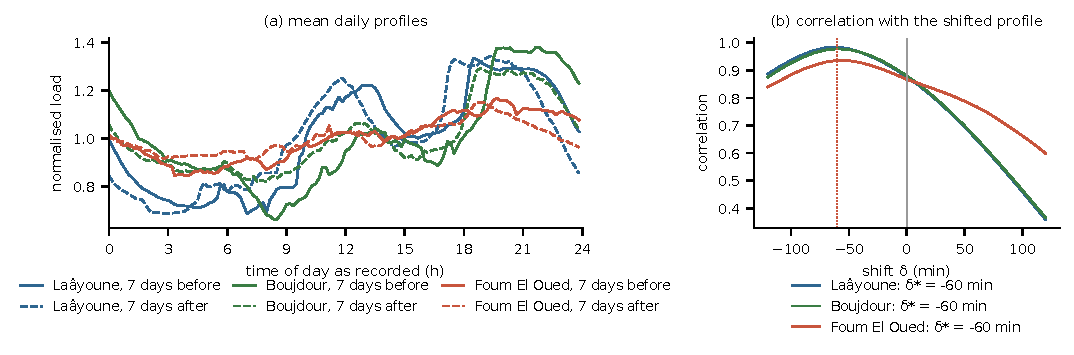
\includegraphics[width=\textwidth]{figures/FigS2}
\caption{Clock evidence at 30 October 2022, the European return to winter time, when the hour 02:00--02:50 is recorded twice. (a) Mean daily profile of each southern city over the 7 days before (solid) and after (dashed) the date, normalised by its mean; (b) correlation of the two profiles as a function of the shift applied to the second: $\delta^{*} = -60$~min in all three cities.}\label{fig:s-clock}
\end{sfigure}

\begin{stable}
\caption{Candidate load-transfer days: the rule items of kind transfer. On each day, the 14-day median of one zone's daily mean current rises and another's falls, each by more than 25\% of the zone's mean level ($\Delta$: median of the 14 days after minus median of the 14 days ending on the day). The conservation index $\kappa = |\sum_z \Delta_z| / \max(\Delta_{\mathrm{up}}, -\Delta_{\mathrm{down}})$ is computed over all zones of the city; rule R16 votes G5 when $\kappa \leq 0.3$. Fig.~\ref{fig:s-transfer} shows the only conserved transfer.}\label{tab:s-transfers}
\footnotesize\setlength{\tabcolsep}{4pt}
\begin{tabular}{@{}l l l l r l@{}}
\toprule
Day & City & Zone up ($\Delta$, A) & Zone down ($\Delta$, A) & $\kappa$ & Final label (confidence) \\
\midrule
2022-10-07 & Foum El Oued & F4 (15.6) & F2 (-35.2) & 0.97 & N (0.98) \\
2022-12-12 & Foum El Oued & F6 (9.7) & F7 (-35.5) & 3.93 & N (0.98) \\
2022-12-18 & Foum El Oued & F6 (9.3) & F2 (-45.2) & 4.15 & N (0.98) \\
2022-12-19 & Foum El Oued & F6 (8.3) & F3 (-44.7) & 3.87 & N (0.98) \\
2023-02-21 & Foum El Oued & F3 (34.3) & F6 (-7.6) & 1.85 & N (0.98) \\
2023-02-27 & Foum El Oued & F7 (25.5) & F6 (-6.6) & 1.85 & N (0.98) \\
2023-03-15 & Foum El Oued & F6 (6.5) & F7 (-42.4) & 2.94 & N (0.98) \\
2023-03-24 & Foum El Oued & F6 (10.3) & F1 (-17.7) & 1.45 & N (0.98) \\
2023-04-16 & Foum El Oued & F4 (12.4) & F6 (-8.5) & 0.72 & N (0.98) \\
2023-04-19 & Foum El Oued & F2 (58.2) & F6 (-6.6) & 3.61 & N (0.98) \\
2023-05-03 & Foum El Oued & F6 (9.9) & F2 (-50.4) & 2.99 & N (0.98) \\
2023-11-23 & Foum El Oued & F3 (25.0) & F4 (-11.2) & 2.54 & N (0.98) \\
2023-12-16 & Boujdour & B2 (33.0) & B1 (-31.9) & 0.07 & G5 (0.68) \\
\bottomrule
\end{tabular}
\end{stable}

\begin{sfigure}
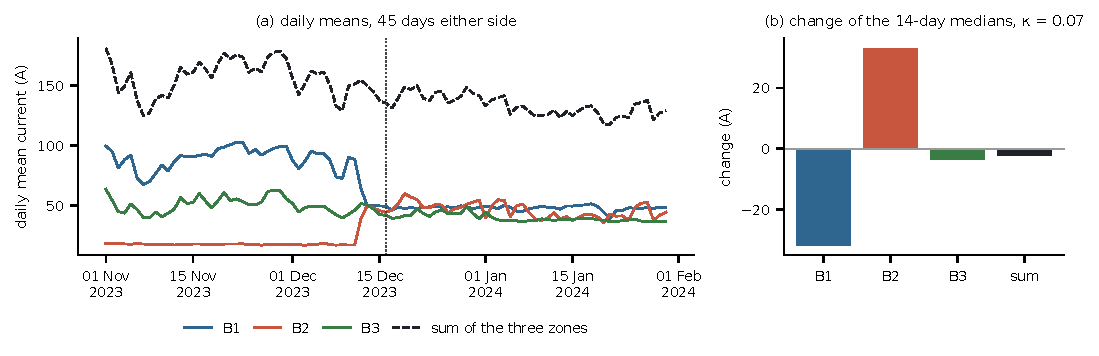
\includegraphics[width=\textwidth]{figures/FigS3}
\caption{The only conserved load transfer: Boujdour, 16 December 2023. (a) Daily mean current of the three zones and their sum over 45 days either side of the day (dotted); (b) change of the 14-day medians: B2 gains what B1 loses, so the city total is conserved ($\kappa = 0.07$, Table~\ref{tab:s-transfers}), and rule R16 votes G5.}\label{fig:s-transfer}
\end{sfigure}

\section{Rules and label model}\label{sec:s-rules}
\begin{stable}
\caption{Learned parameters of the constrained label model on the real data. For each rule: the classes its output speaks for, the items on which it is applicable (its precondition can be observed) and on which it fires, the propensity $a$ (probability of the output when the item's class is one the output speaks for), the false-positive rate $b$ (probability of the output otherwise), the evidence $\ln(a/b)$ and the learned precision (mean posterior mass on the classes the output speaks for, over the items the rule fires on). $^{\dagger}$Defining rule, with the prior Beta(9, 1) on $a$ instead of Beta(1, 1). R7 never fires on the real data and has no row.}\label{tab:s-rule-params}
\scriptsize\setlength{\tabcolsep}{4pt}
\begin{tabular}{@{}l l c l r r r r r r@{}}
\toprule
Rule & Family & Output & Speaks for & Applicable & Fired & $a$ & $b$ & $\ln(a/b)$ & Learned \\
 & & & & items & & & & & precision \\
\midrule
R1 & simultaneity & A1 & A1 & 126 & 1 & 0.4034 & 0.0075 & 3.99 & 1.000 \\
R2$^{\dagger}$ & holds & A2 & A2 & 70 & 12 & 0.6360 & 0.0193 & 3.50 & 0.991 \\
R3 & holds & A1 & A1 & 126 & 3 & 0.6045 & 0.0151 & 3.69 & 0.666 \\
R4 & holds & A1 & A1 & 126 & 3 & 0.4035 & 0.0225 & 2.89 & 0.333 \\
R5 & restoration & G & G1--G5 & 126 & 21 & 0.1684 & 0.1497 & 0.12 & 0.955 \\
R6 & restoration & G & G1--G5 & 126 & 84 & 0.6797 & 0.0775 & 2.17 & 1.000 \\
R8$^{\dagger}$ & city & G2 & G2 & 126 & 1 & 0.9090 & 0.0075 & 4.80 & 0.994 \\
R9 & single zone & G3 & G3, G4 & 126 & 122 & 0.9919 & 0.0733 & 2.61 & 1.000 \\
R10$^{\dagger}$ & calendar & G4 & G4 & 126 & 69 & 0.8925 & 0.0563 & 2.76 & 0.964 \\
R11 & single zone & G3 & G3 & 126 & 4 & 0.0996 & 0.0122 & 2.10 & 0.978 \\
R12$^{\dagger}$ & holds & A3 & A3 & 70 & 44 & 0.9543 & 0.0308 & 3.43 & 0.999 \\
R13$^{\dagger}$ & clock & A4 & A4 & 19 & 8 & 0.9232 & 0.0755 & 2.50 & 0.925 \\
R14$^{\dagger}$ & calendar & A4 & A4 & 14 & 6 & 0.8827 & 0.1468 & 1.79 & 0.701 \\
R15 & clock & A4 & A4 & 32 & 6 & 0.4306 & 0.0574 & 2.02 & 0.886 \\
R16$^{\dagger}$ & conservation & G5 & G5 & 13 & 1 & 0.8899 & 0.0596 & 2.70 & 0.681 \\
R19$^{\dagger}$ & straight-line fills & A2 & A2 & 101 & 48 & 0.9513 & 0.0178 & 3.98 & 0.998 \\
R20$^{\dagger}$ & straight-line fills & A3 & A3 & 101 & 48 & 0.9588 & 0.0169 & 4.04 & 0.999 \\
R21 & straight-line fills & A1 & A1 & 126 & 5 & 0.3908 & 0.0381 & 2.33 & 0.188 \\
\bottomrule
\end{tabular}
\end{stable}

\begin{sfigure}
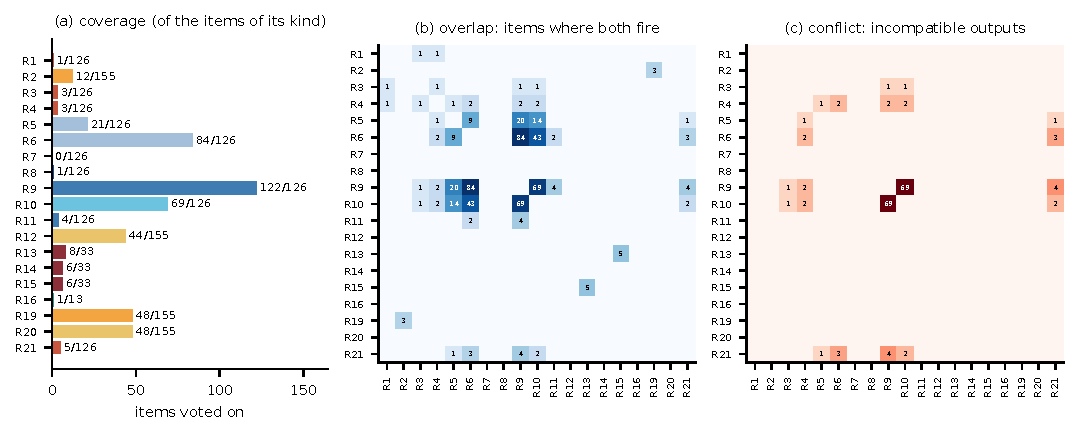
\includegraphics[width=\textwidth]{figures/FigS4}
\caption{Rule diagnostics on the real data. (a) Items each rule votes on, out of the items of the kind it reads, coloured by the rule's output; (b) items on which two rules both fire; (c) items on which two rules give incompatible outputs. Colour scales are logarithmic.}\label{fig:s-rules}
\end{sfigure}

\begin{stable}
\caption{Stability of the labels on the real data (327 rule items). Agreement: share of items whose label equals the label of the kept restart (Dawid--Skene models; the restart with the highest penalised log-likelihood is kept) or of seed~0 (Snorkel). The constrained and unconstrained models restrict every item to its feasible set $\mathcal{Y}(i)$; Snorkel's label model does not. Snorkel's labels agree with ours on 0.755 of the items.}\label{tab:s-stability}
\footnotesize\setlength{\tabcolsep}{4pt}
\begin{tabular}{@{}l l r r r@{}}
\toprule
Label model & Runs & Agreement, min & Agreement, mean & Labels outside $\mathcal{Y}(i)$ \\
\midrule
Constrained label model (ours) & 20 restarts & 1.000 & 1.000 & 0 \\
Unconstrained Dawid--Skene model & 20 restarts & 0.627 & 0.832 & 0 \\
Snorkel label model & 20 seeds & 0.847 & 0.961 & 6 \\
\bottomrule
\end{tabular}
\end{stable}

\begin{stable}
\caption{Recovery of known classes. Classes and votes are simulated for the 327 real items from the fitted constrained model, the label models are refitted on the simulated votes, and the recovered labels are scored against the simulated classes (mean $\pm$ s.d. over the simulation runs; ECE with 10 equal-width bins).}\label{tab:s-recovery}
\footnotesize\setlength{\tabcolsep}{4pt}
\begin{tabular}{@{}l c c c c@{}}
\toprule
Labeller & Accuracy & Macro-F1 & ECE & Brier score \\
\midrule
Constrained label model (ours) & 0.922 $\pm$ 0.021 & 0.872 $\pm$ 0.080 & 0.033 $\pm$ 0.012 & 0.124 $\pm$ 0.028 \\
Unconstrained Dawid--Skene model & 0.682 $\pm$ 0.058 & 0.493 $\pm$ 0.077 & 0.276 $\pm$ 0.065 & 0.577 $\pm$ 0.118 \\
Majority vote & 0.911 $\pm$ 0.017 & 0.843 $\pm$ 0.064 & -- & -- \\
\bottomrule
\end{tabular}
\end{stable}

\begin{stable}
\caption{Sensitivity of the real-data labels to every rule family and prior: the share of items whose label changes when one rule family is removed or one prior or initial value is changed, over all 327 items and per item kind (126 dead, 155 fill, 33 clock, 13 transfer). The simultaneity family includes R7, which never fires.}\label{tab:s-robustness}
\footnotesize\setlength{\tabcolsep}{4pt}
\begin{tabular}{@{}l r r r r r@{}}
\toprule
Change & All items & Dead & Fill & Clock & Transfer \\
\midrule
without the calendar rules (R10, R14) & 17.1\% & 38.9\% & 0.0\% & 21.2\% & 0.0\% \\
without the city rules (R8) & 0.3\% & 0.8\% & 0.0\% & 0.0\% & 0.0\% \\
without the clock rules (R13, R15) & 2.4\% & 0.0\% & 0.0\% & 24.2\% & 0.0\% \\
without the conservation rules (R16) & 3.7\% & 0.0\% & 0.0\% & 0.0\% & 92.3\% \\
without the hold rules (R2, R3, R4, R12) & 0.6\% & 0.0\% & 1.3\% & 0.0\% & 0.0\% \\
without the straight-line-fill rules (R19, R20, R21) & 46.8\% & 0.8\% & 98.1\% & 0.0\% & 0.0\% \\
without the restoration rules (R5, R6) & 0.0\% & 0.0\% & 0.0\% & 0.0\% & 0.0\% \\
without the simultaneity rules (R1, R7) & 0.0\% & 0.0\% & 0.0\% & 0.0\% & 0.0\% \\
without the single-zone rules (R9, R11) & 0.0\% & 0.0\% & 0.0\% & 0.0\% & 0.0\% \\
\midrule
prior Beta(1, 4) on $b$ (default Beta(1, 9)) & 1.8\% & 0.0\% & 0.0\% & 18.2\% & 0.0\% \\
prior Beta(1, 19) on $b$ & 0.0\% & 0.0\% & 0.0\% & 0.0\% & 0.0\% \\
no defining-rule prior (Beta(1, 1) on every $a$) & 16.2\% & 38.9\% & 1.9\% & 3.0\% & 0.0\% \\
class-prior pseudo-count $\gamma$ = 0.5 (default 1) & 0.9\% & 0.0\% & 1.9\% & 0.0\% & 0.0\% \\
class-prior pseudo-count $\gamma$ = 2 & 0.9\% & 0.0\% & 1.9\% & 0.0\% & 0.0\% \\
initial $a$ = 0.9, $b$ = 0.02 (default 0.7, 0.05) & 0.0\% & 0.0\% & 0.0\% & 0.0\% & 0.0\% \\
\bottomrule
\end{tabular}
\end{stable}

\section{Detector and end model on the real data}\label{sec:s-detector}
\begin{stable}
\caption{Accuracy of the predictors of $\rho = x/\hat{x}$ on the real southern data, on rule-clean zone-steps, out of sample (two-fold temporal cross-fitting split at 1 July 2023). Median: median absolute error. The nowcast reads, besides the forecast features, the current value of every other zone (a fully connected input with no learned edges). Corrections are added to the LightGBM forecast by a TCN without or with the learned graph.}\label{tab:s-predictors}
\footnotesize\setlength{\tabcolsep}{4pt}
\begin{tabular}{@{}l r r r r r r@{}}
\toprule
 & \multicolumn{3}{c}{Whole record} & \multicolumn{3}{c}{From 1 July 2023} \\
\cmidrule(lr){2-4}\cmidrule(lr){5-7}
Predictor & MAE & Median & RMSE & MAE & Median & RMSE \\
\midrule
LightGBM forecast (the LightGBM residual) & 0.0288 & 0.0164 & 0.0541 & 0.0278 & 0.0160 & 0.0493 \\
LightGBM nowcast & 0.0292 & 0.0167 & 0.0548 & 0.0282 & 0.0165 & 0.0494 \\
TCN without the graph & 0.0299 & 0.0189 & 0.0498 & 0.0289 & 0.0175 & 0.0494 \\
TCN-GAT (main detector) & 0.0294 & 0.0181 & 0.0497 & 0.0296 & 0.0177 & 0.0504 \\
LightGBM + TCN correction (no graph) & 0.0288 & 0.0163 & 0.0542 & 0.0278 & 0.0161 & 0.0494 \\
LightGBM + learned-graph correction & 0.0288 & 0.0164 & 0.0541 & 0.0278 & 0.0160 & 0.0492 \\
Mean of LightGBM and TCN-GAT & 0.0282 & 0.0166 & 0.0496 & 0.0278 & 0.0161 & 0.0486 \\
\bottomrule
\end{tabular}
\end{stable}

\begin{stable}
\caption{Event formation chosen on the development datasets (3\% with seeds 100--102, 1\% with seed 103, 7\% with seed 104): for each detector, the best of the 48 settings of the smoothing window $w$ (steps), the percentile $q$ and the merge gap $g_{\max}$ (steps) by mean event F1 of the detector alone. F1, untuned setting: the same detector with $(w, q, g_{\max}) = (1, 99.5\%, 1)$. Real-data candidates: detector-only candidates on the uninjected southern series at the chosen setting (events that do not overlap a rule item). The main detector was chosen among the four predictors by the development F1 of the rules plus its candidates. GDN, USAD and the main detector without the graph are tuned the same way; their settings are given in Tables~\ref{tab:s-deep} and \ref{tab:s-graph}.}\label{tab:s-dev}
\scriptsize\setlength{\tabcolsep}{3.5pt}
\begin{tabular}{@{}l r r r r r r r r r@{}}
\toprule
Detector & $w$ & $q$ & $g_{\max}$ & F1 & Precision & Recall & Zone-strict & F1, untuned & Real-data \\
 & & & & & & & F1 & setting & candidates \\
\midrule
Isolation Forest & 3 & 99.5\% & 3 & 0.473 & 0.412 & 0.599 & 0.419 & 0.384 & 416 \\
LOF & 24 & 99.8\% & 12 & 0.648 & 0.726 & 0.621 & 0.615 & 0.464 & 148 \\
LightGBM + learned-graph correction & 24 & 99.8\% & 6 & 0.760 & 0.826 & 0.714 & 0.732 & 0.683 & 56 \\
LightGBM residual & 24 & 99.8\% & 6 & 0.759 & 0.828 & 0.710 & 0.731 & 0.681 & 58 \\
STL & 24 & 99.8\% & 12 & 0.717 & 0.846 & 0.628 & 0.680 & 0.591 & 86 \\
Main detector & 24 & 99.9\% & 12 & 0.786 & 0.866 & 0.729 & 0.755 & 0.649 & 70 \\
Mean of LightGBM and TCN-GAT & 48 & 99.8\% & 12 & 0.771 & 0.861 & 0.703 & 0.729 & 0.672 & 44 \\
\bottomrule
\end{tabular}
\end{stable}

\begin{stable}
\caption{Alarms of the detectors alone on the real southern data by day type: the share of rule-negative zone-steps (no rule state of the zone within $\pm$53 steps) whose score exceeds the detector's threshold, and its ratio to the rate on ordinary weekdays. Day types are exclusive, in the order Eid, national holiday, Ramadan, weekend.}\label{tab:s-hard-negatives}
\scriptsize\setlength{\tabcolsep}{4pt}
\begin{tabular}{@{}l l r r r@{}}
\toprule
Detector & Day type & Zone-steps & Flag rate & Ratio to ordinary weekdays \\
\midrule
Main detector & ordinary weekday & 746,257 & 0.0011 & 1.00 \\
 & weekend & 288,425 & 0.0019 & 1.70 \\
 & Ramadan & 116,548 & 0.0008 & 0.73 \\
 & national holiday & 29,970 & 0.0011 & 0.99 \\
 & Eid & 11,280 & 0.0028 & 2.56 \\
\midrule
Mean of LightGBM and TCN-GAT & ordinary weekday & 746,425 & 0.0020 & 1.00 \\
 & weekend & 288,425 & 0.0025 & 1.28 \\
 & Ramadan & 116,548 & 0.0027 & 1.35 \\
 & national holiday & 29,970 & 0.0000 & 0.00 \\
 & Eid & 11,280 & 0.0027 & 1.39 \\
\midrule
LightGBM + learned-graph correction & ordinary weekday & 746,257 & 0.0018 & 1.00 \\
 & weekend & 288,425 & 0.0021 & 1.16 \\
 & Ramadan & 116,548 & 0.0041 & 2.29 \\
 & national holiday & 29,970 & 0.0000 & 0.00 \\
 & Eid & 11,280 & 0.0007 & 0.39 \\
\midrule
LightGBM + TCN correction (no graph) & ordinary weekday & 746,257 & 0.0011 & 1.00 \\
 & weekend & 288,425 & 0.0013 & 1.24 \\
 & Ramadan & 116,548 & 0.0002 & 0.17 \\
 & national holiday & 29,970 & 0.0000 & 0.00 \\
 & Eid & 11,280 & 0.0000 & 0.00 \\
\midrule
LightGBM residual & ordinary weekday & 746,257 & 0.0018 & 1.00 \\
 & weekend & 288,425 & 0.0021 & 1.17 \\
 & Ramadan & 116,548 & 0.0039 & 2.15 \\
 & national holiday & 29,970 & 0.0000 & 0.00 \\
 & Eid & 11,280 & 0.0006 & 0.34 \\
\bottomrule
\end{tabular}
\end{stable}

\begin{sfigure}
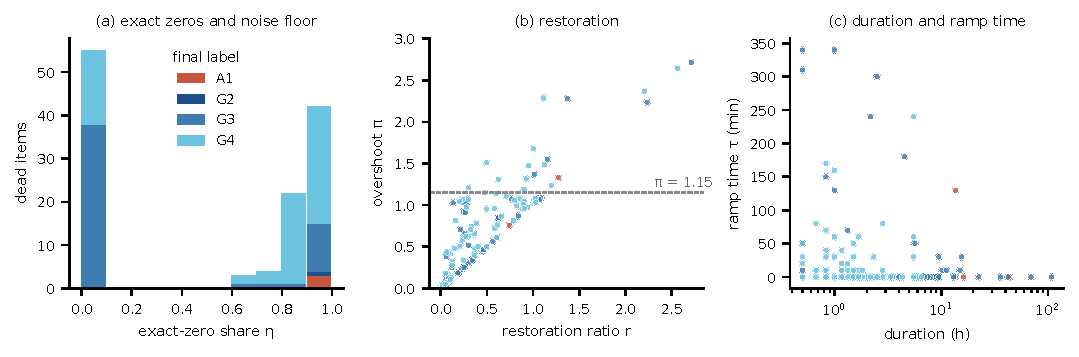
\includegraphics[width=\textwidth]{figures/FigS5}
\caption{Signatures of the 126 dead items of the real data, coloured by final label. (a) Share of exact zeros $\eta$ in the dead run; (b) restoration ratio $r$ and overshoot $\pi$ (dashed: the threshold of rule R5); (c) duration and ramp time $\tau$. The restoration features do not separate the classes.}\label{fig:s-signatures}
\end{sfigure}

\begin{sfigure}
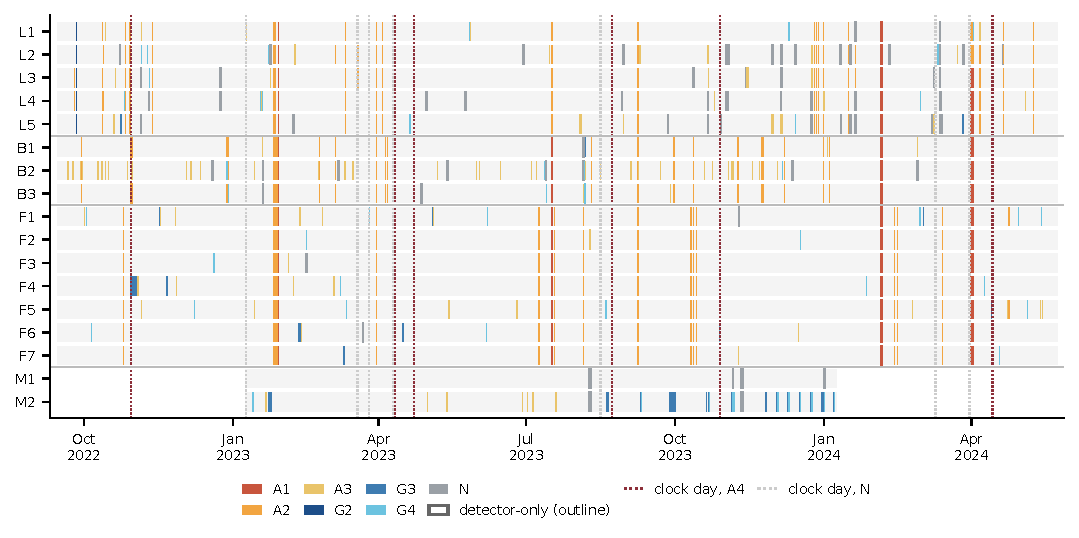
\includegraphics[width=\textwidth]{figures/FigS6}
\caption{The typed catalogue on one timeline: rule items of kind dead and fill (filled) and detector-only candidates (outlined) per zone, coloured by final label; dotted lines: clock days (coloured when labelled A4).}\label{fig:s-timeline}
\end{sfigure}

\begin{sfigure}
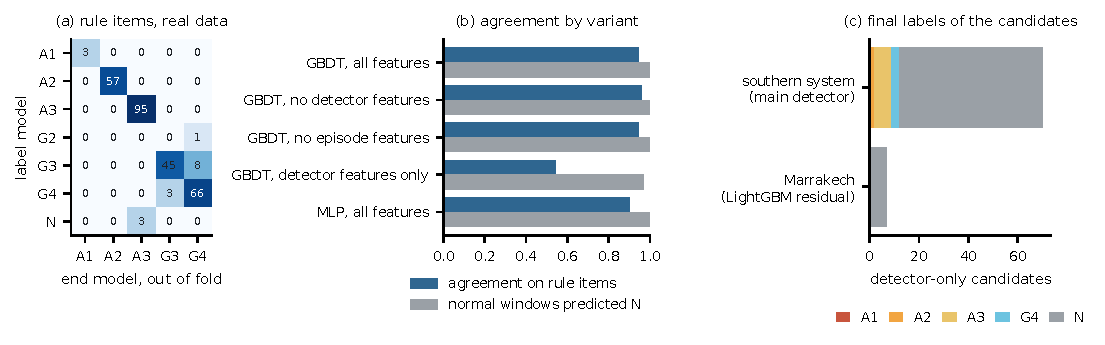
\includegraphics[width=\textwidth]{figures/FigS7}
\caption{End model on the real data. (a) Label-model label against the out-of-fold end-model label of the rule items; (b) agreement with the label model on the rule items and share of normal windows predicted N, by variant (GBDT: gradient-boosted trees); (c) final labels of the detector-only candidates, from the main detector in the southern system and from the LightGBM residual in Marrakech.}\label{fig:s-endmodel}
\end{sfigure}

\section{Injection benchmark}\label{sec:s-benchmark}
\begin{figure}[htbp]
\centering
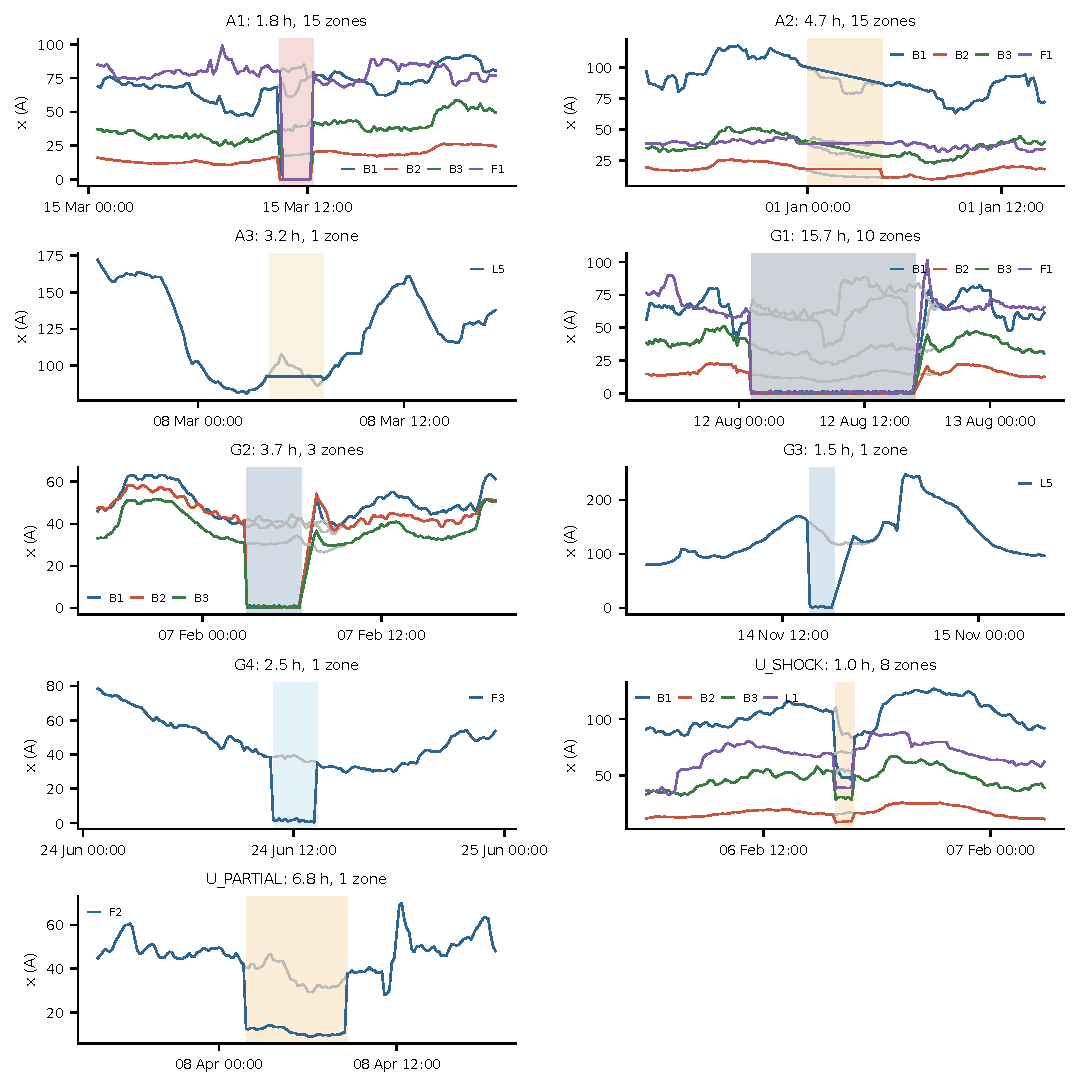
\includegraphics[width=\textwidth]{figures/FigS8}
\caption{One injected event of each type over the original series (grey), from the dataset with 3\% contamination and seed~0; shading: the injected span. U\_SHOCK and U\_PARTIAL scale the load down and are not typed by any rule.}\label{fig:s-injected}
\end{figure}

\begingroup\scriptsize\setlength{\tabcolsep}{3.2pt}
\begin{longtable}{@{}l >{\raggedright\arraybackslash}p{3.9cm} rrrrrrrrr@{}}
\caption{Recall by injected type (share of the injected events of the type that overlap a predicted event), test period, mean over the 10 test seeds. U\_SHOCK and U\_PARTIAL are untyped events that no rule can see. Untuned event formation: $(w, q, g_{\max}) = (1, 99.5\%, 1)$. The nowcast is defined in Table~\ref{tab:s-predictors}.}\label{tab:s-recall}\\
\toprule
Rate & Method & A1 & A2 & A3 & G1 & G2 & G3 & G4 & U\_SHOCK & U\_PARTIAL \\
\midrule
\endfirsthead
\multicolumn{11}{@{}l}{\emph{Table \thetable, continued}}\\
\toprule
Rate & Method & A1 & A2 & A3 & G1 & G2 & G3 & G4 & U\_SHOCK & U\_PARTIAL \\
\midrule
\endhead
\bottomrule
\endfoot
1\% & Full method & 1.000 & 1.000 & 1.000 & 1.000 & 1.000 & 1.000 & 1.000 & 0.302 & 0.180 \\
 & Rules alone & 1.000 & 1.000 & 1.000 & 1.000 & 0.900 & 1.000 & 1.000 & 0.000 & 0.000 \\
 & Main detector & 1.000 & 0.888 & 0.252 & 1.000 & 1.000 & 1.000 & 0.975 & 0.302 & 0.180 \\
 & Main detector, untuned event formation & 1.000 & 0.967 & 0.507 & 1.000 & 1.000 & 1.000 & 1.000 & 0.925 & 0.534 \\
 & Main detector, raw band only & 1.000 & 0.930 & 0.302 & 1.000 & 1.000 & 1.000 & 1.000 & 0.142 & 0.148 \\
 & LightGBM residual & 1.000 & 0.838 & 0.148 & 1.000 & 1.000 & 0.975 & 0.926 & 0.130 & 0.213 \\
 & LightGBM residual, untuned event formation & 1.000 & 0.967 & 0.457 & 1.000 & 1.000 & 1.000 & 1.000 & 0.753 & 0.406 \\
 & LightGBM + learned-graph correction & 1.000 & 0.838 & 0.132 & 1.000 & 1.000 & 0.975 & 0.926 & 0.130 & 0.233 \\
 & LightGBM + TCN correction (no graph) & 1.000 & 0.677 & 0.082 & 1.000 & 0.780 & 0.938 & 0.824 & 0.010 & 0.107 \\
 & Mean of LightGBM and TCN-GAT & 1.000 & 0.838 & 0.148 & 1.000 & 1.000 & 0.975 & 0.926 & 0.078 & 0.127 \\
 & LightGBM nowcast, raw band & 0.960 & 0.618 & 0.000 & 1.000 & 0.685 & 0.905 & 0.804 & 0.000 & 0.050 \\
\midrule
3\% & Full method & 1.000 & 1.000 & 1.000 & 1.000 & 1.000 & 1.000 & 1.000 & 0.212 & 0.207 \\
 & Rules alone & 1.000 & 1.000 & 1.000 & 1.000 & 0.929 & 1.000 & 1.000 & 0.000 & 0.020 \\
 & Main detector & 1.000 & 0.788 & 0.289 & 1.000 & 0.994 & 1.000 & 1.000 & 0.212 & 0.207 \\
 & Main detector, untuned event formation & 1.000 & 0.862 & 0.437 & 1.000 & 1.000 & 1.000 & 1.000 & 0.774 & 0.395 \\
 & Main detector, raw band only & 1.000 & 0.820 & 0.312 & 1.000 & 1.000 & 1.000 & 1.000 & 0.111 & 0.231 \\
 & LightGBM residual & 1.000 & 0.725 & 0.215 & 1.000 & 0.973 & 0.947 & 0.915 & 0.163 & 0.162 \\
 & LightGBM residual, untuned event formation & 1.000 & 0.855 & 0.360 & 1.000 & 1.000 & 1.000 & 1.000 & 0.591 & 0.320 \\
 & LightGBM + learned-graph correction & 1.000 & 0.731 & 0.208 & 1.000 & 0.973 & 0.947 & 0.915 & 0.169 & 0.162 \\
 & LightGBM + TCN correction (no graph) & 0.992 & 0.608 & 0.147 & 1.000 & 0.894 & 0.896 & 0.841 & 0.023 & 0.133 \\
 & Mean of LightGBM and TCN-GAT & 1.000 & 0.736 & 0.177 & 1.000 & 0.955 & 0.939 & 0.925 & 0.038 & 0.163 \\
 & LightGBM nowcast, raw band & 0.975 & 0.580 & 0.071 & 1.000 & 0.788 & 0.831 & 0.726 & 0.000 & 0.066 \\
\midrule
7\% & Full method & 1.000 & 1.000 & 1.000 & 1.000 & 0.998 & 1.000 & 1.000 & 0.052 & 0.220 \\
 & Rules alone & 1.000 & 1.000 & 1.000 & 1.000 & 0.939 & 1.000 & 1.000 & 0.000 & 0.000 \\
 & Main detector & 0.997 & 0.726 & 0.255 & 1.000 & 0.998 & 0.997 & 0.987 & 0.058 & 0.220 \\
 & Main detector, untuned event formation & 0.997 & 0.768 & 0.292 & 1.000 & 1.000 & 1.000 & 0.997 & 0.285 & 0.283 \\
 & Main detector, raw band only & 0.997 & 0.782 & 0.314 & 1.000 & 1.000 & 0.994 & 1.000 & 0.053 & 0.236 \\
 & LightGBM residual & 0.988 & 0.648 & 0.184 & 1.000 & 0.975 & 0.908 & 0.938 & 0.045 & 0.205 \\
 & LightGBM residual, untuned event formation & 0.997 & 0.766 & 0.280 & 1.000 & 1.000 & 0.982 & 0.991 & 0.192 & 0.287 \\
 & LightGBM + learned-graph correction & 0.988 & 0.650 & 0.187 & 1.000 & 0.975 & 0.906 & 0.938 & 0.045 & 0.204 \\
 & LightGBM + TCN correction (no graph) & 0.959 & 0.573 & 0.119 & 1.000 & 0.872 & 0.832 & 0.844 & 0.018 & 0.140 \\
 & Mean of LightGBM and TCN-GAT & 0.993 & 0.675 & 0.195 & 1.000 & 0.966 & 0.912 & 0.960 & 0.028 & 0.196 \\
 & LightGBM nowcast, raw band & 0.940 & 0.535 & 0.069 & 1.000 & 0.828 & 0.792 & 0.780 & 0.015 & 0.103 \\
\end{longtable}
\endgroup

\begingroup\scriptsize\setlength{\tabcolsep}{4pt}
\begin{longtable}{@{}l l l r r r@{}}
\caption{Paired two-sided Wilcoxon signed-rank tests over the 10 test seeds on event F1 (Section~5.3 of the article; every predicted event counts, alarms on the uninjected series included). The smallest attainable $p$ is 0.002. With the method's own alarms on the uninjected series excluded, the full method beats the rules alone in 10 of 10 seeds at every rate ($p = 0.002$).}\label{tab:s-detection-tests}\\
\toprule
Rate & Method & Compared with & F1, method & F1, other & $p$ \\
\midrule
\endfirsthead
\multicolumn{6}{@{}l}{\emph{Table \thetable, continued}}\\
\toprule
Rate & Method & Compared with & F1, method & F1, other & $p$ \\
\midrule
\endhead
\bottomrule
\endfoot
1\% & Full method & Rules alone & 0.721 & 0.863 & 0.002 \\
3\% & Full method & Rules alone & 0.876 & 0.879 & 0.625 \\
7\% & Full method & Rules alone & 0.906 & 0.896 & 0.002 \\
\midrule
1\% & Main detector & Mean of LightGBM and TCN-GAT & 0.644 & 0.655 & 0.557 \\
1\% & Main detector & LightGBM + learned-graph correction & 0.644 & 0.627 & 0.322 \\
1\% & Main detector & LightGBM + TCN correction (no graph) & 0.644 & 0.645 & 1.000 \\
1\% & Main detector & LightGBM residual & 0.644 & 0.623 & 0.160 \\
1\% & Main detector & STL & 0.644 & 0.625 & 0.492 \\
1\% & Main detector & Isolation Forest & 0.644 & 0.211 & 0.002 \\
1\% & Main detector & LOF & 0.644 & 0.570 & 0.010 \\
3\% & Main detector & Mean of LightGBM and TCN-GAT & 0.813 & 0.773 & 0.002 \\
3\% & Main detector & LightGBM + learned-graph correction & 0.813 & 0.765 & 0.002 \\
3\% & Main detector & LightGBM + TCN correction (no graph) & 0.813 & 0.752 & 0.002 \\
3\% & Main detector & LightGBM residual & 0.813 & 0.765 & 0.002 \\
3\% & Main detector & STL & 0.813 & 0.734 & 0.002 \\
3\% & Main detector & Isolation Forest & 0.813 & 0.462 & 0.002 \\
3\% & Main detector & LOF & 0.813 & 0.720 & 0.002 \\
7\% & Main detector & Mean of LightGBM and TCN-GAT & 0.854 & 0.843 & 0.020 \\
7\% & Main detector & LightGBM + learned-graph correction & 0.854 & 0.827 & 0.004 \\
7\% & Main detector & LightGBM + TCN correction (no graph) & 0.854 & 0.790 & 0.002 \\
7\% & Main detector & LightGBM residual & 0.854 & 0.827 & 0.002 \\
7\% & Main detector & STL & 0.854 & 0.771 & 0.002 \\
7\% & Main detector & Isolation Forest & 0.854 & 0.605 & 0.002 \\
7\% & Main detector & LOF & 0.854 & 0.698 & 0.002 \\
\end{longtable}
\endgroup

\begin{stable}
\caption{The deep multivariate baselines GDN and USAD on the injection benchmark (test period, mean $\pm$ s.d. over the 10 test seeds), with their own event formation tuned on the development datasets, and their recall by injected type (means; F1 with their own alarms excluded and their real-data alarms are in Table~6 of the article). GDN finds the multi-city zero gaps (A1) but almost none of the single-zone fills (A3).}\label{tab:s-deep}
\scriptsize\setlength{\tabcolsep}{2pt}
\begin{tabular}{@{}l l l l l l rrrrrrr@{}}
\toprule
Method & Rate & $(w, q, g_{\max})$ & F1 & Precision & Recall & \multicolumn{7}{c}{Recall by type (mean)} \\
\cmidrule(l){7-13}
 & & & & & & A1 & A2 & A3 & G1 & G2 & G3 & G4 \\
\midrule
GDN & 1\% & w 6, q 99.5, gap 1 & 0.370 $\pm$ 0.044 & 0.268 $\pm$ 0.041 & 0.602 $\pm$ 0.053 & 0.990 & 0.270 & 0.000 & 1.000 & 0.755 & 0.776 & 0.554 \\
GDN & 3\% & w 6, q 99.5, gap 1 & 0.563 $\pm$ 0.028 & 0.519 $\pm$ 0.021 & 0.617 $\pm$ 0.050 & 0.977 & 0.291 & 0.014 & 1.000 & 0.821 & 0.564 & 0.502 \\
GDN & 7\% & w 6, q 99.5, gap 1 & 0.707 $\pm$ 0.025 & 0.776 $\pm$ 0.035 & 0.650 $\pm$ 0.030 & 0.956 & 0.248 & 0.014 & 1.000 & 0.742 & 0.562 & 0.571 \\
\midrule
USAD & 1\% & w 6, q 99.0, gap 3 & 0.286 $\pm$ 0.046 & 0.233 $\pm$ 0.047 & 0.378 $\pm$ 0.058 & 0.636 & 0.153 & 0.000 & 0.933 & 0.400 & 0.405 & 0.258 \\
USAD & 3\% & w 6, q 99.0, gap 3 & 0.413 $\pm$ 0.025 & 0.485 $\pm$ 0.043 & 0.362 $\pm$ 0.033 & 0.666 & 0.106 & 0.000 & 0.922 & 0.301 & 0.221 & 0.213 \\
USAD & 7\% & w 6, q 99.0, gap 3 & 0.517 $\pm$ 0.038 & 0.759 $\pm$ 0.029 & 0.393 $\pm$ 0.043 & 0.631 & 0.082 & 0.011 & 0.877 & 0.355 & 0.265 & 0.244 \\
\bottomrule
\end{tabular}
\end{stable}

\begin{stable}
\caption{GDN's one-step forecasts against two naive forecasts on clean windows of the real southern series, for the two cross-fitted models (mean squared error of $\rho$). On clean data GDN's forecasts are 7--14 times worse than the last value.}\label{tab:s-gdn-forecast}
\scriptsize\setlength{\tabcolsep}{4pt}
\begin{tabular}{@{}l l r r r r r@{}}
\toprule
GDN trained on & Windows & $n$ & MSE, GDN & MSE, last value & MSE, mean of & Ratio GDN / \\
 & & & & & last 5 values & last value \\
\midrule
before 1 July 2023 & training fold (in sample) & 38,249 & 0.00419 & 0.00035 & 0.00075 & 11.9 \\
before 1 July 2023 & other fold (out of sample) & 45,222 & 0.00490 & 0.00035 & 0.00072 & 13.8 \\
from 1 July 2023 & training fold (in sample) & 45,222 & 0.00267 & 0.00037 & 0.00073 & 7.3 \\
from 1 July 2023 & other fold (out of sample) & 38,249 & 0.00251 & 0.00038 & 0.00077 & 6.7 \\
\bottomrule
\end{tabular}
\end{stable}

\begingroup\scriptsize\setlength{\tabcolsep}{4pt}
\begin{longtable}{@{}l l l r r r r@{}}
\caption{Paired two-sided Wilcoxon tests of the deep baselines on event F1 (10 test seeds). Other better: seeds in which the compared method has the higher F1.}\label{tab:s-deep-tests}\\
\toprule
Rate & Baseline & Compared with & F1, baseline & F1, other & Other better & $p$ \\
\midrule
\endfirsthead
\multicolumn{7}{@{}l}{\emph{Table \thetable, continued}}\\
\toprule
Rate & Baseline & Compared with & F1, baseline & F1, other & Other better & $p$ \\
\midrule
\endhead
\bottomrule
\endfoot
1\% & GDN & Main detector & 0.3701 & 0.6438 & 10/10 & 0.002 \\
1\% & GDN & Rules alone & 0.3701 & 0.8631 & 10/10 & 0.002 \\
1\% & GDN & Full method & 0.3701 & 0.7209 & 10/10 & 0.002 \\
1\% & GDN & STL & 0.3701 & 0.6249 & 10/10 & 0.002 \\
1\% & GDN & Isolation Forest & 0.3701 & 0.2107 & 0/10 & 0.002 \\
1\% & GDN & LOF & 0.3701 & 0.5696 & 10/10 & 0.002 \\
1\% & USAD & Main detector & 0.2864 & 0.6438 & 10/10 & 0.002 \\
1\% & USAD & Rules alone & 0.2864 & 0.8631 & 10/10 & 0.002 \\
1\% & USAD & Full method & 0.2864 & 0.7209 & 10/10 & 0.002 \\
1\% & USAD & STL & 0.2864 & 0.6249 & 10/10 & 0.002 \\
1\% & USAD & Isolation Forest & 0.2864 & 0.2107 & 0/10 & 0.002 \\
1\% & USAD & LOF & 0.2864 & 0.5696 & 10/10 & 0.002 \\
\midrule
3\% & GDN & Main detector & 0.5628 & 0.8131 & 10/10 & 0.002 \\
3\% & GDN & Rules alone & 0.5628 & 0.8794 & 10/10 & 0.002 \\
3\% & GDN & Full method & 0.5628 & 0.8755 & 10/10 & 0.002 \\
3\% & GDN & STL & 0.5628 & 0.7345 & 10/10 & 0.002 \\
3\% & GDN & Isolation Forest & 0.5628 & 0.4619 & 0/10 & 0.002 \\
3\% & GDN & LOF & 0.5628 & 0.7198 & 10/10 & 0.002 \\
3\% & USAD & Main detector & 0.4126 & 0.8131 & 10/10 & 0.002 \\
3\% & USAD & Rules alone & 0.4126 & 0.8794 & 10/10 & 0.002 \\
3\% & USAD & Full method & 0.4126 & 0.8755 & 10/10 & 0.002 \\
3\% & USAD & STL & 0.4126 & 0.7345 & 10/10 & 0.002 \\
3\% & USAD & Isolation Forest & 0.4126 & 0.4619 & 8/10 & 0.027 \\
3\% & USAD & LOF & 0.4126 & 0.7198 & 10/10 & 0.002 \\
\midrule
7\% & GDN & Main detector & 0.7069 & 0.8540 & 10/10 & 0.002 \\
7\% & GDN & Rules alone & 0.7069 & 0.8959 & 10/10 & 0.002 \\
7\% & GDN & Full method & 0.7069 & 0.9057 & 10/10 & 0.002 \\
7\% & GDN & STL & 0.7069 & 0.7713 & 10/10 & 0.002 \\
7\% & GDN & Isolation Forest & 0.7069 & 0.6053 & 2/10 & 0.010 \\
7\% & GDN & LOF & 0.7069 & 0.6976 & 8/10 & 0.432 \\
7\% & USAD & Main detector & 0.5167 & 0.8540 & 10/10 & 0.002 \\
7\% & USAD & Rules alone & 0.5167 & 0.8959 & 10/10 & 0.002 \\
7\% & USAD & Full method & 0.5167 & 0.9057 & 10/10 & 0.002 \\
7\% & USAD & STL & 0.5167 & 0.7713 & 10/10 & 0.002 \\
7\% & USAD & Isolation Forest & 0.5167 & 0.6053 & 9/10 & 0.014 \\
7\% & USAD & LOF & 0.5167 & 0.6976 & 9/10 & 0.004 \\
\end{longtable}
\endgroup

\begingroup\scriptsize\setlength{\tabcolsep}{3.5pt}
\begin{longtable}{@{}l >{\raggedright\arraybackslash}p{4.4cm} l l r r r r@{}}
\caption{Ablations of the main detector (the numbers behind Fig.~8 of the article): event F1 (mean $\pm$ s.d. over the 10 test seeds), the mean $\pm$ s.d. of the per-seed difference from the main detector, the paired Wilcoxon $p$, the seeds in which the main detector is better, F1 with the detector's own alarms on the uninjected series excluded, and step-wise AUC-PR. $\Delta$F1 is rounded from the unrounded per-seed differences.}\label{tab:s-ablations}\\
\toprule
Rate & Variant & Event F1 & $\Delta$F1 vs main & $p$ & Main & F1, own & AUC-PR \\
 & & & & & better & background excl. & \\
\midrule
\endfirsthead
\multicolumn{8}{@{}l}{\emph{Table \thetable, continued}}\\
\toprule
Rate & Variant & Event F1 & $\Delta$F1 vs main & $p$ & Main & F1, own & AUC-PR \\
 & & & & & better & background excl. & \\
\midrule
\endhead
\bottomrule
\endfoot
1\% & Main detector & 0.644 $\pm$ 0.067 & -- & -- & -- & 0.817 & 0.547 \\
1\% & without the learned graph, same event formation & 0.671 $\pm$ 0.048 & $+$0.0270 $\pm$ 0.0326 & 0.037 & 2/10 & 0.826 & 0.540 \\
1\% & without the learned graph, own event formation & 0.707 $\pm$ 0.040 & $+$0.0630 $\pm$ 0.0447 & 0.004 & 1/10 & 0.823 & 0.505 \\
1\% & without the graph and the bands (TCN, raw band) & 0.612 $\pm$ 0.053 & $-$0.0316 $\pm$ 0.0369 & 0.027 & 8/10 & 0.825 & 0.591 \\
1\% & without the bands (raw band only) & 0.595 $\pm$ 0.046 & $-$0.0484 $\pm$ 0.0357 & 0.004 & 9/10 & 0.789 & 0.566 \\
1\% & without the hierarchy (flat zone score) & 0.675 $\pm$ 0.040 & $+$0.0312 $\pm$ 0.0629 & 0.160 & 3/10 & 0.823 & 0.736 \\
1\% & LightGBM predictor (own event formation) & 0.623 $\pm$ 0.055 & $-$0.0208 $\pm$ 0.0490 & 0.160 & 7/10 & 0.793 & 0.592 \\
1\% & untuned event formation (1, 99.5\%, 1) & 0.365 $\pm$ 0.063 & $-$0.2787 $\pm$ 0.0401 & 0.002 & 10/10 & 0.805 & 0.541 \\
\midrule
3\% & Main detector & 0.813 $\pm$ 0.020 & -- & -- & -- & 0.842 & 0.598 \\
3\% & without the learned graph, same event formation & 0.817 $\pm$ 0.020 & $+$0.0040 $\pm$ 0.0076 & 0.131 & 3/10 & 0.847 & 0.598 \\
3\% & without the learned graph, own event formation & 0.801 $\pm$ 0.019 & $-$0.0119 $\pm$ 0.0142 & 0.020 & 9/10 & 0.829 & 0.574 \\
3\% & without the graph and the bands (TCN, raw band) & 0.775 $\pm$ 0.021 & $-$0.0378 $\pm$ 0.0162 & 0.002 & 10/10 & 0.842 & 0.668 \\
3\% & without the bands (raw band only) & 0.772 $\pm$ 0.017 & $-$0.0412 $\pm$ 0.0148 & 0.002 & 10/10 & 0.834 & 0.626 \\
3\% & without the hierarchy (flat zone score) & 0.796 $\pm$ 0.014 & $-$0.0173 $\pm$ 0.0184 & 0.014 & 9/10 & 0.841 & 0.811 \\
3\% & LightGBM predictor (own event formation) & 0.765 $\pm$ 0.022 & $-$0.0484 $\pm$ 0.0222 & 0.002 & 10/10 & 0.817 & 0.678 \\
3\% & untuned event formation (1, 99.5\%, 1) & 0.670 $\pm$ 0.040 & $-$0.1434 $\pm$ 0.0386 & 0.002 & 10/10 & 0.812 & 0.595 \\
\midrule
7\% & Main detector & 0.854 $\pm$ 0.011 & -- & -- & -- & 0.848 & 0.565 \\
7\% & without the learned graph, same event formation & 0.857 $\pm$ 0.009 & $+$0.0029 $\pm$ 0.0039 & 0.064 & 3/10 & 0.852 & 0.568 \\
7\% & without the learned graph, own event formation & 0.861 $\pm$ 0.012 & $+$0.0066 $\pm$ 0.0069 & 0.027 & 2/10 & 0.856 & 0.532 \\
7\% & without the graph and the bands (TCN, raw band) & 0.864 $\pm$ 0.010 & $+$0.0100 $\pm$ 0.0066 & 0.004 & 1/10 & 0.862 & 0.634 \\
7\% & without the bands (raw band only) & 0.853 $\pm$ 0.011 & $-$0.0005 $\pm$ 0.0074 & 0.846 & 5/10 & 0.853 & 0.598 \\
7\% & without the hierarchy (flat zone score) & 0.856 $\pm$ 0.011 & $+$0.0022 $\pm$ 0.0078 & 0.375 & 4/10 & 0.862 & 0.791 \\
7\% & LightGBM predictor (own event formation) & 0.827 $\pm$ 0.015 & $-$0.0272 $\pm$ 0.0139 & 0.002 & 10/10 & 0.830 & 0.633 \\
7\% & untuned event formation (1, 99.5\%, 1) & 0.835 $\pm$ 0.010 & $-$0.0185 $\pm$ 0.0053 & 0.002 & 10/10 & 0.828 & 0.572 \\
\end{longtable}
\endgroup

\begin{stable}
\caption{The learned graph as an ablation: the main detector with and without the graph attention, the latter at the main detector's event formation (w 24, q 99.9, gap 12) and at its own, tuned on the development datasets like every detector (w 48, q 99.9, gap 12). Event F1: mean $\pm$ s.d. over the 10 test seeds; the other columns: means.}\label{tab:s-graph}
\scriptsize\setlength{\tabcolsep}{2.2pt}
\begin{tabular}{@{}l l l r r r r r r r r@{}}
\toprule
Rate & Variant & F1 & Precision & Recall & Zone- & AUC-PR & F1, own & Real-data & U\_SHOCK & U\_PARTIAL \\
 & & & & & strict F1 & & bg.\ excl. & alarms & recall & recall \\
\midrule
1\% & with graph & 0.644 $\pm$ 0.067 & 0.583 & 0.730 & 0.615 & 0.547 & 0.817 & 191 & 0.302 & 0.180 \\
1\% & no graph & 0.671 $\pm$ 0.048 & 0.614 & 0.747 & 0.641 & 0.540 & 0.826 & 202 & 0.277 & 0.213 \\
1\% & no graph, own & 0.707 $\pm$ 0.040 & 0.696 & 0.722 & 0.675 & 0.505 & 0.823 & 170 & 0.253 & 0.181 \\
\midrule
3\% & with graph & 0.813 $\pm$ 0.020 & 0.892 & 0.748 & 0.783 & 0.598 & 0.842 & 191 & 0.212 & 0.207 \\
3\% & no graph & 0.817 $\pm$ 0.020 & 0.887 & 0.758 & 0.789 & 0.598 & 0.847 & 202 & 0.255 & 0.206 \\
3\% & no graph, own & 0.801 $\pm$ 0.019 & 0.881 & 0.735 & 0.765 & 0.574 & 0.829 & 170 & 0.123 & 0.215 \\
\midrule
7\% & with graph & 0.854 $\pm$ 0.011 & 0.976 & 0.759 & 0.805 & 0.565 & 0.848 & 191 & 0.058 & 0.220 \\
7\% & no graph & 0.857 $\pm$ 0.009 & 0.974 & 0.765 & 0.806 & 0.568 & 0.852 & 202 & 0.076 & 0.233 \\
7\% & no graph, own & 0.861 $\pm$ 0.012 & 0.975 & 0.770 & 0.800 & 0.532 & 0.856 & 170 & 0.028 & 0.264 \\
\bottomrule
\end{tabular}
\end{stable}

\begin{stable}
\caption{Detector variants at 3\% contamination (test period, mean $\pm$ s.d. over the 10 test seeds), at the main detector's event formation unless stated; recall columns: means.}\label{tab:s-variants}
\scriptsize\setlength{\tabcolsep}{3.5pt}
\begin{tabular}{@{}>{\raggedright\arraybackslash}p{4.8cm} l l r r r r@{}}
\toprule
Variant & Event F1 & AUC-PR & A2 & G3 & U\_SHOCK & U\_PARTIAL \\
 & & & recall & recall & recall & recall \\
\midrule
Main detector & 0.813 $\pm$ 0.020 & 0.598 $\pm$ 0.044 & 0.788 & 1.000 & 0.212 & 0.207 \\
Mean of LightGBM and TCN-GAT & 0.773 $\pm$ 0.024 & 0.592 $\pm$ 0.055 & 0.736 & 0.939 & 0.038 & 0.163 \\
LightGBM + learned-graph correction & 0.765 $\pm$ 0.024 & 0.676 $\pm$ 0.056 & 0.731 & 0.947 & 0.169 & 0.162 \\
LightGBM + TCN correction (no graph) & 0.752 $\pm$ 0.026 & 0.671 $\pm$ 0.056 & 0.608 & 0.896 & 0.023 & 0.133 \\
LightGBM residual & 0.765 $\pm$ 0.022 & 0.678 $\pm$ 0.053 & 0.725 & 0.947 & 0.163 & 0.162 \\
Main detector, untuned event formation & 0.670 $\pm$ 0.040 & 0.595 $\pm$ 0.041 & 0.862 & 1.000 & 0.774 & 0.395 \\
LightGBM residual, untuned event formation & 0.705 $\pm$ 0.036 & 0.695 $\pm$ 0.049 & 0.855 & 1.000 & 0.591 & 0.320 \\
Main detector, raw band only & 0.772 $\pm$ 0.017 & 0.626 $\pm$ 0.042 & 0.820 & 1.000 & 0.111 & 0.231 \\
Main detector, no hierarchy (flat zone score) & 0.796 $\pm$ 0.014 & 0.811 $\pm$ 0.042 & 0.836 & 1.000 & 0.053 & 0.222 \\
LightGBM nowcast, raw band & 0.715 $\pm$ 0.022 & 0.704 $\pm$ 0.054 & 0.580 & 0.831 & 0.000 & 0.066 \\
TCN without the graph, raw band & 0.775 $\pm$ 0.021 & 0.668 $\pm$ 0.050 & 0.821 & 1.000 & 0.196 & 0.245 \\
\bottomrule
\end{tabular}
\end{stable}

\begin{stable}
\caption{Sensitivity to the rule-engine thresholds on injected data (3\%, test seeds 0--2, test period; mean $\pm$ s.d.): the rules alone and the label model with one threshold changed at a time; recall columns: means.}\label{tab:s-thresholds}
\scriptsize\setlength{\tabcolsep}{3pt}
\begin{tabular}{@{}>{\raggedright\arraybackslash}p{3.9cm} l r r r r r r l@{}}
\toprule
Thresholds & Rules & Rules & A2 & A3 & G3 & G4 & U\_PARTIAL & Label model \\
 & F1 & recall & recall & recall & recall & recall & recall & macro-F1 \\
\midrule
as used ($\varepsilon$ 0.05, hold 6, $\tau$ 10 min) & 0.891 $\pm$ 0.012 & 0.803 & 1.000 & 1.000 & 1.000 & 1.000 & 0.042 & 0.906 $\pm$ 0.020 \\
noise floor $\varepsilon$ = 0.02 & 0.880 $\pm$ 0.006 & 0.786 & 1.000 & 1.000 & 0.946 & 0.944 & 0.000 & 0.819 $\pm$ 0.014 \\
noise floor $\varepsilon$ = 0.10 & 0.881 $\pm$ 0.015 & 0.812 & 1.000 & 1.000 & 1.000 & 1.000 & 0.162 & 0.915 $\pm$ 0.023 \\
hold of 4 equal values & 0.765 $\pm$ 0.007 & 0.803 & 1.000 & 1.000 & 1.000 & 1.000 & 0.042 & 0.906 $\pm$ 0.020 \\
hold of 12 equal values & 0.880 $\pm$ 0.011 & 0.786 & 0.972 & 0.820 & 1.000 & 1.000 & 0.042 & 0.885 $\pm$ 0.017 \\
simultaneity window $\tau$ = 0 min & 0.891 $\pm$ 0.012 & 0.803 & 1.000 & 1.000 & 1.000 & 1.000 & 0.042 & 0.905 $\pm$ 0.024 \\
simultaneity window $\tau$ = 20 min & 0.891 $\pm$ 0.012 & 0.803 & 1.000 & 1.000 & 1.000 & 1.000 & 0.042 & 0.904 $\pm$ 0.022 \\
\bottomrule
\end{tabular}
\end{stable}

\begin{stable}
\caption{The label model refitted without one rule family at a time, on the typed injected events detected by the full method (3\%, test period, mean $\pm$ s.d. over the 10 test seeds).}\label{tab:s-families}
\footnotesize\setlength{\tabcolsep}{4pt}
\begin{tabular}{@{}l l@{}}
\toprule
Label model & Macro-F1 \\
\midrule
all rule families & 0.914 $\pm$ 0.029 \\
without the calendar rules & 0.778 $\pm$ 0.021 \\
without the city rules & 0.922 $\pm$ 0.029 \\
without the conservation rules & 0.915 $\pm$ 0.026 \\
without the hold rules & 0.893 $\pm$ 0.032 \\
without the straight-line-fill rules & 0.724 $\pm$ 0.110 \\
without the restoration rules & 0.902 $\pm$ 0.029 \\
without the simultaneity rules & 0.941 $\pm$ 0.047 \\
without the single-zone rules & 0.915 $\pm$ 0.028 \\
\bottomrule
\end{tabular}
\end{stable}

\begin{stable}
\caption{Attribution against the rules' majority vote (the tests behind Table~7 of the article): macro-F1 on the typed injected events detected by the full method (test period, mean over the 10 test seeds), the seeds in which the labeller is better, tied or worse, and the paired Wilcoxon $p$. Fusion weight $\beta$ tuned on the earlier period: 0.7, 0.6, 0.6 at 1, 3 and 7\%; the end model abstains on classes with fewer than 3 training items.}\label{tab:s-attribution-tests}
\footnotesize\setlength{\tabcolsep}{4pt}
\begin{tabular}{@{}l l r r c r@{}}
\toprule
Rate & Labeller & Macro-F1 & Macro-F1, majority vote & Better / tied / worse & $p$ \\
\midrule
1\% & Label model & 0.9345 & 0.9397 & 1 / 6 / 3 & 0.144 \\
1\% & Fusion & 0.9442 & 0.9397 & 3 / 6 / 1 & 0.465 \\
3\% & Label model & 0.9142 & 0.9209 & 2 / 0 / 8 & 0.131 \\
3\% & Fusion & 0.9194 & 0.9209 & 5 / 2 / 3 & 0.889 \\
7\% & Label model & 0.9003 & 0.9134 & 1 / 0 / 9 & 0.006 \\
7\% & Fusion & 0.9064 & 0.9134 & 3 / 0 / 7 & 0.131 \\
\bottomrule
\end{tabular}
\end{stable}

\begin{stable}
\caption{Snorkel's label model on the same rule votes (injected data, the typed events matched by a rule item; macro-F1, mean $\pm$ s.d. over the 10 test seeds), and paired Wilcoxon tests of our label model against each labeller (lower block: mean macro-F1, seeds in which ours is better and tied). Feasible sets: Snorkel's probabilities restricted to the item's feasible classes.}\label{tab:s-snorkel}
\scriptsize\setlength{\tabcolsep}{4pt}
\begin{tabular}{@{}l r l l l l@{}}
\toprule
Rate & Events & Majority vote & Label model (ours) & Snorkel & Snorkel + feasible sets \\
\midrule
1\% & 309 & 0.950 $\pm$ 0.044 & 0.946 $\pm$ 0.040 & 0.903 $\pm$ 0.050 & 0.903 $\pm$ 0.050 \\
3\% & 895 & 0.929 $\pm$ 0.028 & 0.923 $\pm$ 0.026 & 0.898 $\pm$ 0.031 & 0.898 $\pm$ 0.031 \\
7\% & 2,503 & 0.919 $\pm$ 0.015 & 0.907 $\pm$ 0.021 & 0.874 $\pm$ 0.030 & 0.878 $\pm$ 0.030 \\
\midrule
1\% &  & ours vs majority vote & 0.9464 vs 0.9500 & ours better in 0, tied in 9 & $p$ = 0.317 \\
1\% &  & ours vs Snorkel & 0.9464 vs 0.9032 & ours better in 9, tied in 1 & $p$ = 0.008 \\
1\% &  & ours vs Snorkel + feasible sets & 0.9464 vs 0.9032 & ours better in 9, tied in 1 & $p$ = 0.008 \\
3\% &  & ours vs majority vote & 0.9227 vs 0.9289 & ours better in 1, tied in 5 & $p$ = 0.138 \\
3\% &  & ours vs Snorkel & 0.9227 vs 0.8981 & ours better in 8, tied in 0 & $p$ = 0.020 \\
3\% &  & ours vs Snorkel + feasible sets & 0.9227 vs 0.8981 & ours better in 8, tied in 0 & $p$ = 0.020 \\
7\% &  & ours vs majority vote & 0.9072 vs 0.9188 & ours better in 2, tied in 1 & $p$ = 0.021 \\
7\% &  & ours vs Snorkel & 0.9072 vs 0.8735 & ours better in 8, tied in 0 & $p$ = 0.010 \\
7\% &  & ours vs Snorkel + feasible sets & 0.9072 vs 0.8779 & ours better in 8, tied in 0 & $p$ = 0.010 \\
\bottomrule
\end{tabular}
\end{stable}

\section{Downstream test}\label{sec:s-downstream}
\begingroup\scriptsize\setlength{\tabcolsep}{3.2pt}
\begin{longtable}{@{}l l l l r r r r r r r r@{}}
\caption{Forecasting on the 30 injected test datasets by rate (the numbers behind Table~8 and Fig.~10 of the article): mean MASE of each cleaning strategy, test period 1 January -- 24 May 2024, on steps within two days after an anomalous state (after) or all scored steps (all); the datasets in which S2 has the lower MASE and the paired Wilcoxon $p$. Naive: persistence at 1~h, seasonal naive at 1~day.}\label{tab:s-forecast30}\\
\toprule
Forecaster & Horizon & Steps & Rate & S0 & S1 & S2 & S3 & S2 better & $p$ & S2 better & $p$ \\
 & & & & \multicolumn{4}{c}{MASE (mean)} & than S1 & & than S0 & \\
\midrule
\endfirsthead
\multicolumn{12}{@{}l}{\emph{Table \thetable, continued}}\\
\toprule
Forecaster & Horizon & Steps & Rate & S0 & S1 & S2 & S3 & S2 better & $p$ & S2 better & $p$ \\
 & & & & \multicolumn{4}{c}{MASE (mean)} & than S1 & & than S0 & \\
\midrule
\endhead
\bottomrule
\endfoot
LightGBM & 1 day & after & 1\% & 1.323 & 1.206 & 1.069 & 1.068 & 10/10 & 0.002 & 10/10 & 0.002 \\
LightGBM & 1 day & after & 3\% & 1.290 & 1.134 & 1.078 & 1.063 & 9/10 & 0.037 & 9/10 & 0.004 \\
LightGBM & 1 day & after & 7\% & 1.273 & 1.081 & 1.027 & 1.023 & 10/10 & 0.002 & 10/10 & 0.002 \\
LightGBM & 1 day & after & all & 1.295 & 1.140 & 1.058 & 1.052 & 29/30 & $<$0.001 & 29/30 & $<$0.001 \\
LightGBM & 1 day & all & 1\% & 1.122 & 1.090 & 1.069 & 1.070 & 10/10 & 0.002 & 10/10 & 0.002 \\
LightGBM & 1 day & all & 3\% & 1.160 & 1.085 & 1.067 & 1.065 & 9/10 & 0.084 & 10/10 & 0.002 \\
LightGBM & 1 day & all & 7\% & 1.240 & 1.054 & 1.019 & 1.018 & 10/10 & 0.002 & 10/10 & 0.002 \\
LightGBM & 1 day & all & all & 1.174 & 1.076 & 1.052 & 1.051 & 29/30 & $<$0.001 & 30/30 & $<$0.001 \\
\midrule
LightGBM & 1 h & after & 1\% & 0.683 & 0.655 & 0.629 & 0.626 & 10/10 & 0.002 & 10/10 & 0.002 \\
LightGBM & 1 h & after & 3\% & 0.693 & 0.632 & 0.638 & 0.637 & 9/10 & 0.084 & 9/10 & 0.084 \\
LightGBM & 1 h & after & 7\% & 0.712 & 0.621 & 0.607 & 0.595 & 10/10 & 0.002 & 10/10 & 0.002 \\
LightGBM & 1 h & after & all & 0.696 & 0.636 & 0.625 & 0.619 & 29/30 & $<$0.001 & 29/30 & $<$0.001 \\
LightGBM & 1 h & all & 1\% & 0.640 & 0.635 & 0.629 & 0.627 & 10/10 & 0.002 & 10/10 & 0.002 \\
LightGBM & 1 h & all & 3\% & 0.651 & 0.631 & 0.645 & 0.642 & 9/10 & 0.084 & 9/10 & 0.084 \\
LightGBM & 1 h & all & 7\% & 0.669 & 0.610 & 0.601 & 0.589 & 9/10 & 0.004 & 10/10 & 0.002 \\
LightGBM & 1 h & all & all & 0.653 & 0.625 & 0.625 & 0.620 & 28/30 & $<$0.001 & 29/30 & $<$0.001 \\
\midrule
naive & 1 day & after & 1\% & 2.117 & 1.476 & 1.436 & 1.429 & 8/10 & 0.105 & 10/10 & 0.002 \\
naive & 1 day & after & 3\% & 2.113 & 1.389 & 1.524 & 1.457 & 2/10 & 0.014 & 10/10 & 0.002 \\
naive & 1 day & after & 7\% & 1.878 & 1.268 & 1.538 & 1.457 & 0/10 & 0.002 & 10/10 & 0.002 \\
naive & 1 day & after & all & 2.036 & 1.377 & 1.499 & 1.448 & 10/30 & 0.001 & 30/30 & $<$0.001 \\
naive & 1 day & all & 1\% & 1.233 & 1.148 & 1.142 & 1.141 & 8/10 & 0.084 & 10/10 & 0.002 \\
naive & 1 day & all & 3\% & 1.351 & 1.165 & 1.202 & 1.184 & 2/10 & 0.014 & 10/10 & 0.002 \\
naive & 1 day & all & 7\% & 1.484 & 1.165 & 1.305 & 1.263 & 0/10 & 0.002 & 10/10 & 0.002 \\
naive & 1 day & all & all & 1.356 & 1.159 & 1.216 & 1.196 & 10/30 & 0.001 & 30/30 & $<$0.001 \\
\midrule
naive & 1 h & after & 1\% & 1.020 & 0.970 & 0.979 & 0.972 & 0/10 & 0.002 & 10/10 & 0.002 \\
naive & 1 h & after & 3\% & 0.998 & 0.921 & 0.940 & 0.926 & 0/10 & 0.002 & 10/10 & 0.002 \\
naive & 1 h & after & 7\% & 0.965 & 0.868 & 0.898 & 0.872 & 0/10 & 0.002 & 10/10 & 0.002 \\
naive & 1 h & after & all & 0.994 & 0.920 & 0.939 & 0.923 & 0/30 & $<$0.001 & 30/30 & $<$0.001 \\
naive & 1 h & all & 1\% & 0.929 & 0.922 & 0.923 & 0.922 & 0/10 & 0.002 & 10/10 & 0.002 \\
naive & 1 h & all & 3\% & 0.921 & 0.901 & 0.906 & 0.902 & 0/10 & 0.002 & 10/10 & 0.002 \\
naive & 1 h & all & 7\% & 0.899 & 0.848 & 0.863 & 0.850 & 0/10 & 0.002 & 10/10 & 0.002 \\
naive & 1 h & all & all & 0.916 & 0.890 & 0.898 & 0.891 & 0/30 & $<$0.001 & 30/30 & $<$0.001 \\
\end{longtable}
\endgroup

\begin{stable}
\caption{Diebold--Mariano tests per injected dataset (30 datasets): the number of datasets in which S2 is significantly better or worse ($p < 0.05$) and the mean statistic (positive: S2 better).}\label{tab:s-dm30}
\scriptsize\setlength{\tabcolsep}{4pt}
\begin{tabular}{@{}l l l l r r r@{}}
\toprule
Forecaster & Horizon & Steps & Comparison & S2 significantly better & S2 significantly worse & Mean DM \\
\midrule
LightGBM & 1 day & after & S0 vs S2 & 19 & 0 & 3.18 \\
LightGBM & 1 day & after & S1 vs S2 & 14 & 0 & 1.89 \\
LightGBM & 1 day & all & S0 vs S2 & 26 & 0 & 4.77 \\
LightGBM & 1 day & all & S1 vs S2 & 19 & 0 & 2.21 \\
LightGBM & 1 h & after & S0 vs S2 & 28 & 1 & 4.60 \\
LightGBM & 1 h & after & S1 vs S2 & 26 & 1 & 3.67 \\
LightGBM & 1 h & all & S0 vs S2 & 29 & 1 & 5.54 \\
LightGBM & 1 h & all & S1 vs S2 & 25 & 1 & 4.00 \\
naive & 1 day & after & S0 vs S2 & 21 & 0 & 2.35 \\
naive & 1 day & after & S1 vs S2 & 0 & 11 & -1.34 \\
naive & 1 day & all & S0 vs S2 & 21 & 0 & 2.33 \\
naive & 1 day & all & S1 vs S2 & 0 & 11 & -1.34 \\
naive & 1 h & after & S0 vs S2 & 24 & 0 & 2.89 \\
naive & 1 h & after & S1 vs S2 & 0 & 21 & -2.24 \\
naive & 1 h & all & S0 vs S2 & 24 & 0 & 2.88 \\
naive & 1 h & all & S1 vs S2 & 0 & 21 & -2.24 \\
\bottomrule
\end{tabular}
\end{stable}

\begingroup\scriptsize\setlength{\tabcolsep}{4pt}
\begin{longtable}{@{}l l l l r r r r r@{}}
\caption{Diebold--Mariano tests on the real data (test period 1 January -- 24 May 2024): loss summed over zones, $d_t = L^{(1)}_t - L^{(2)}_t$ (positive: the second strategy better), Newey--West variance with bandwidth equal to the horizon.}\label{tab:s-dm-real}\\
\toprule
Forecaster & Horizon & Steps & Comparison & $n$ & Mean loss & Share of steps & DM & $p$ \\
 & & & & & difference & second better & & \\
\midrule
\endfirsthead
\multicolumn{9}{@{}l}{\emph{Table \thetable, continued}}\\
\toprule
Forecaster & Horizon & Steps & Comparison & $n$ & Mean loss & Share of steps & DM & $p$ \\
 & & & & & difference & second better & & \\
\midrule
\endhead
\bottomrule
\endfoot
LightGBM & 1 day & after & S1 vs S2 & 7,725 & 0.553 & 0.506 & 1.22 & 0.222 \\
LightGBM & 1 day & after & S0 vs S2 & 7,725 & 1.411 & 0.505 & 1.19 & 0.233 \\
LightGBM & 1 day & all & S1 vs S2 & 20,448 & 0.204 & 0.502 & 1.16 & 0.247 \\
LightGBM & 1 day & all & S0 vs S2 & 20,448 & 0.567 & 0.508 & 1.26 & 0.209 \\
LightGBM & 1 h & after & S1 vs S2 & 7,725 & 0.155 & 0.538 & 4.94 & $<$0.001 \\
LightGBM & 1 h & after & S0 vs S2 & 7,725 & 0.138 & 0.530 & 3.79 & $<$0.001 \\
LightGBM & 1 h & all & S1 vs S2 & 20,448 & 0.043 & 0.508 & 2.35 & 0.019 \\
LightGBM & 1 h & all & S0 vs S2 & 20,448 & 0.003 & 0.489 & 0.17 & 0.863 \\
naive & 1 day & after & S1 vs S2 & 7,719 & 0.882 & 0.055 & 1.41 & 0.159 \\
naive & 1 day & after & S0 vs S2 & 7,719 & 3.019 & 0.061 & 1.37 & 0.170 \\
naive & 1 day & all & S1 vs S2 & 20,442 & 0.333 & 0.021 & 1.39 & 0.163 \\
naive & 1 day & all & S0 vs S2 & 20,442 & 1.140 & 0.023 & 1.36 & 0.175 \\
naive & 1 h & after & S1 vs S2 & 7,719 & 0.025 & 0.010 & 0.77 & 0.442 \\
naive & 1 h & after & S0 vs S2 & 7,719 & 0.094 & 0.012 & 1.96 & 0.049 \\
naive & 1 h & all & S1 vs S2 & 20,442 & 0.009 & 0.004 & 0.77 & 0.442 \\
naive & 1 h & all & S0 vs S2 & 20,442 & 0.036 & 0.005 & 1.96 & 0.050 \\
\end{longtable}
\endgroup

\begin{stable}
\caption{Outage statistics on the 30 injected test datasets: counted outage zone-hours relative to the injected truth, naive (every flagged dead state) and typed (dead states inside grid-event items), the datasets in which typed counting is closer to the truth ($|\log r|$) and the paired Wilcoxon $p$.}\label{tab:s-outage30}
\scriptsize\setlength{\tabcolsep}{3.5pt}
\begin{tabular}{@{}l r l l l l r r r@{}}
\toprule
Rate & Datasets & Naive ratio & Range & Typed ratio & Range & Typed & $p$ & True outage \\
 & & (mean $\pm$ s.d.) & & (mean $\pm$ s.d.) & & closer & & zone-hours (mean) \\
\midrule
1\% & 10 & 1.76 $\pm$ 0.46 & 1.20--2.56 & 1.16 $\pm$ 0.36 & 1.00--2.16 & 10/10 & 0.002 & 701.9 \\
3\% & 10 & 2.01 $\pm$ 0.26 & 1.49--2.39 & 1.28 $\pm$ 0.20 & 1.06--1.76 & 10/10 & 0.002 & 1916.6 \\
7\% & 10 & 1.89 $\pm$ 0.13 & 1.64--2.02 & 1.33 $\pm$ 0.07 & 1.21--1.45 & 10/10 & 0.002 & 4422.7 \\
all & 30 & 1.88 $\pm$ 0.32 & 1.20--2.56 & 1.26 $\pm$ 0.24 & 1.00--2.16 & 30/30 & 1.9 $\times 10^{-9}$ & 2347.1 \\
\bottomrule
\end{tabular}
\end{stable}

\section{Transfer test}\label{sec:s-transfer}
\begin{sfigure}
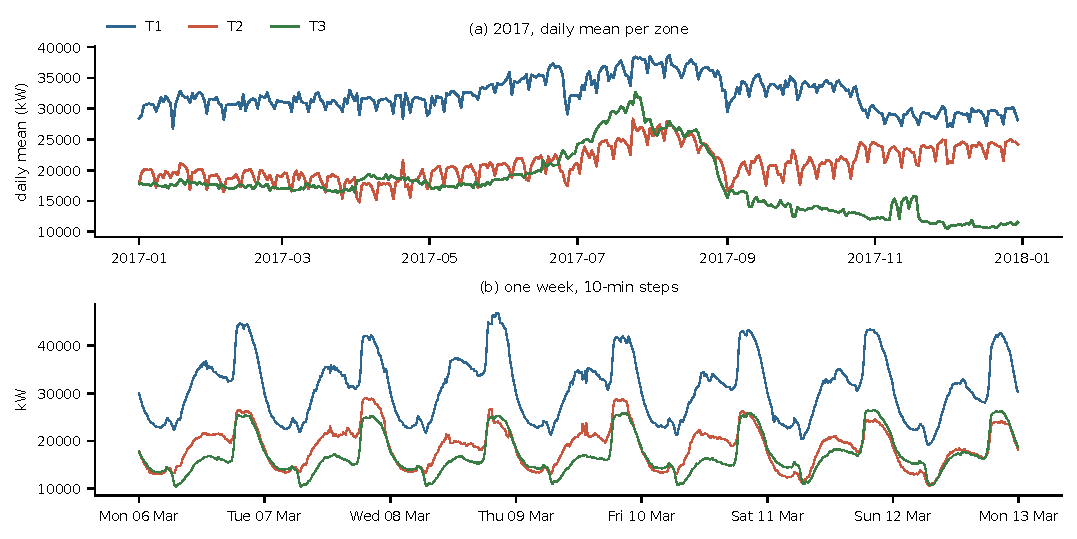
\includegraphics[width=\textwidth]{figures/FigS9}
\caption{The UCI Tetouan data used for the transfer test: three zones of one city, 2017, 10-min steps. (a) Daily mean per zone; (b) one week.}\label{fig:s-tetouan}
\end{sfigure}

\begin{stable}
\caption{Transfer to Tetouan: recall by injected type (mean over the 10 seeds; G1 is not injected in a single-city system).}\label{tab:s-tetouan-recall}
\scriptsize\setlength{\tabcolsep}{3.2pt}
\begin{tabular}{@{}l l rrrrrrrr@{}}
\toprule
Rate & Method & A1 & A2 & A3 & G2 & G3 & G4 & U\_SHOCK & U\_PARTIAL \\
\midrule
1\% & LightGBM residual & 1.000 & 0.863 & 0.350 & 1.000 & 0.950 & 0.975 & 0.200 & 0.900 \\
 & Main detector without the graph & 1.000 & 0.217 & 0.050 & 1.000 & 1.000 & 1.000 & 0.417 & 1.000 \\
 & Main detector & 1.000 & 0.628 & 0.058 & 1.000 & 0.975 & 1.000 & 0.308 & 0.975 \\
 & Full method & 1.000 & 1.000 & 1.000 & 1.000 & 1.000 & 1.000 & 0.308 & 0.975 \\
 & Rules alone & 1.000 & 1.000 & 1.000 & 0.950 & 1.000 & 1.000 & 0.000 & 0.000 \\
\midrule
3\% & LightGBM residual & 1.000 & 0.853 & 0.530 & 1.000 & 0.955 & 0.988 & 0.057 & 0.831 \\
 & Main detector without the graph & 1.000 & 0.287 & 0.012 & 1.000 & 0.978 & 0.962 & 0.069 & 0.761 \\
 & Main detector & 1.000 & 0.416 & 0.009 & 1.000 & 0.976 & 0.950 & 0.020 & 0.736 \\
 & Full method & 1.000 & 1.000 & 1.000 & 1.000 & 1.000 & 1.000 & 0.020 & 0.736 \\
 & Rules alone & 1.000 & 1.000 & 1.000 & 0.951 & 1.000 & 1.000 & 0.000 & 0.000 \\
\midrule
7\% & LightGBM residual & 0.934 & 0.628 & 0.193 & 0.841 & 0.879 & 0.889 & 0.005 & 0.446 \\
 & Main detector without the graph & 0.975 & 0.238 & 0.000 & 0.932 & 0.922 & 0.848 & 0.000 & 0.322 \\
 & Main detector & 0.935 & 0.323 & 0.000 & 0.873 & 0.937 & 0.912 & 0.000 & 0.340 \\
 & Full method & 1.000 & 1.000 & 1.000 & 0.987 & 1.000 & 1.000 & 0.000 & 0.340 \\
 & Rules alone & 0.997 & 1.000 & 1.000 & 0.919 & 1.000 & 1.000 & 0.000 & 0.000 \\
\bottomrule
\end{tabular}
\end{stable}

\begin{stable}
\caption{Transfer to Tetouan: attribution by the frozen label model (one E-step with the parameters fitted on the Moroccan votes) and by the rules' majority vote, mean $\pm$ s.d. over the 10 seeds. End to end: the share of typed injected events both detected and correctly typed.}\label{tab:s-tetouan-attr}
\scriptsize\setlength{\tabcolsep}{4pt}
\begin{tabular}{@{}l l l l l l l@{}}
\toprule
Rate & Typed events & Macro-F1, & Macro-F1, & Accuracy, & Accuracy, & End to end \\
 & detected & label model & majority vote & label model & majority vote & \\
\midrule
1\% & 0.992 $\pm$ 0.026 & 0.793 $\pm$ 0.064 & 0.793 $\pm$ 0.064 & 0.821 $\pm$ 0.062 & 0.821 $\pm$ 0.062 & 0.815 $\pm$ 0.070 \\
3\% & 0.992 $\pm$ 0.010 & 0.774 $\pm$ 0.050 & 0.781 $\pm$ 0.048 & 0.778 $\pm$ 0.044 & 0.781 $\pm$ 0.042 & 0.772 $\pm$ 0.044 \\
7\% & 0.986 $\pm$ 0.007 & 0.771 $\pm$ 0.018 & 0.785 $\pm$ 0.020 & 0.774 $\pm$ 0.018 & 0.780 $\pm$ 0.017 & 0.763 $\pm$ 0.018 \\
\bottomrule
\end{tabular}
\end{stable}

\begingroup\scriptsize\setlength{\tabcolsep}{4pt}
\begin{longtable}{@{}l l r r r r@{}}
\caption{Transfer to Tetouan: paired Wilcoxon tests of the main detector against every other method on event F1 (10 seeds).}\label{tab:s-tetouan-tests}\\
\toprule
Rate & Main detector compared with & F1, main & F1, other & Main better & $p$ \\
\midrule
\endfirsthead
\multicolumn{6}{@{}l}{\emph{Table \thetable, continued}}\\
\toprule
Rate & Main detector compared with & F1, main & F1, other & Main better & $p$ \\
\midrule
\endhead
\bottomrule
\endfoot
1\% & Full method & 0.8570 & 0.9454 & 0/10 & 0.002 \\
1\% & Rules alone & 0.8570 & 0.8564 & 4/10 & 0.889 \\
1\% & Main detector without the graph & 0.8570 & 0.8318 & 7/10 & 0.086 \\
1\% & Main detector without the graph, own event formation & 0.8570 & 0.7987 & 10/10 & 0.002 \\
1\% & LightGBM residual & 0.8570 & 0.7606 & 10/10 & 0.002 \\
1\% & STL & 0.8570 & 0.7467 & 10/10 & 0.002 \\
1\% & Isolation Forest & 0.8570 & 0.4835 & 10/10 & 0.002 \\
1\% & LOF & 0.8570 & 0.7393 & 9/10 & 0.004 \\
\midrule
3\% & Full method & 0.7929 & 0.9189 & 0/10 & 0.002 \\
3\% & Rules alone & 0.7929 & 0.8607 & 0/10 & 0.002 \\
3\% & Main detector without the graph & 0.7929 & 0.7846 & 5/10 & 0.327 \\
3\% & Main detector without the graph, own event formation & 0.7929 & 0.7586 & 9/10 & 0.008 \\
3\% & LightGBM residual & 0.7929 & 0.8682 & 0/10 & 0.002 \\
3\% & STL & 0.7929 & 0.8281 & 1/10 & 0.004 \\
3\% & Isolation Forest & 0.7929 & 0.6920 & 10/10 & 0.002 \\
3\% & LOF & 0.7929 & 0.7282 & 8/10 & 0.064 \\
\midrule
7\% & Full method & 0.7223 & 0.8896 & 0/10 & 0.002 \\
7\% & Rules alone & 0.7223 & 0.8597 & 0/10 & 0.002 \\
7\% & Main detector without the graph & 0.7223 & 0.7120 & 8/10 & 0.131 \\
7\% & Main detector without the graph, own event formation & 0.7223 & 0.6627 & 9/10 & 0.004 \\
7\% & LightGBM residual & 0.7223 & 0.7636 & 1/10 & 0.006 \\
7\% & STL & 0.7223 & 0.7425 & 3/10 & 0.214 \\
7\% & Isolation Forest & 0.7223 & 0.8062 & 0/10 & 0.002 \\
7\% & LOF & 0.7223 & 0.2015 & 10/10 & 0.002 \\
\end{longtable}
\endgroup

\section{Software, settings, run times and seeds}\label{sec:s-repro}
\begin{stable}
\caption{Software and hardware. The versions of the local environment were read on 15 November 2026; each run records the versions it used in its \texttt{summary.json}. LightGBM is pinned at 4.6.0 (4.7.0 crashed on the local machine).}\label{tab:s-software}
\footnotesize\setlength{\tabcolsep}{4pt}
\begin{tabular}{@{}>{\raggedright\arraybackslash}p{4.6cm} >{\raggedright\arraybackslash}p{10.6cm}@{}}
\toprule
Environment & Versions \\
\midrule
Local runs (Windows PC, 8 logical CPU cores) & Python 3.12.1, NumPy 1.26.4, pandas 2.2.0, SciPy 1.12.0, scikit-learn 1.5.1, statsmodels 0.15.0, PyWavelets 1.8.0, Matplotlib 3.8.3, openpyxl 3.1.5 \\
 & LightGBM 4.6.0; PyTorch 2.2.0+cpu on CPU (graph ablation, GDN, USAD) \\
Injection benchmark (NB4) & Google Colab with a GPU (device cuda); PyTorch 2.14.1+cu130, LightGBM 4.6.0 \\
Snorkel baseline & separate environment with Snorkel 0.10.0 \\
\bottomrule
\end{tabular}
\end{stable}

\begin{stable}
\caption{Settings used for every result of the article (the full list of parameters is in the released code). GDN and USAD use the settings released by their authors.}\label{tab:s-settings}
\footnotesize\setlength{\tabcolsep}{4pt}
\begin{tabular}{@{}>{\raggedright\arraybackslash}p{3.3cm} >{\raggedright\arraybackslash}p{12.2cm}@{}}
\toprule
Component & Settings \\
\midrule
Expected value & $\hat{x}$: median of the same time slot over the previous 14 days \\
States & exact zero $x = 0$; noise floor $x \leq 0.05\,\hat{x}$; hold: $\geq 6$ equal values; straight-line fill: $\geq 6$ collinear points \\
Items & runs of one system whose starts lie within $\tau = 10$~min form one item; episodes: items sharing boundaries \\
Label model & priors Beta(1, 1) on $a$ (Beta(9, 1) for defining rules), Beta(1, 9) on $b$, pseudo-count $\gamma = 1$ per class; initial $a = 0.7$, $b = 0.05$; 20 restarts (log-normal jitter, s.d. 0.5); stop at $|\Delta \log L| < 10^{-6}$ or 3,000 iterations; the restart with the highest penalised log-likelihood is kept \\
LightGBM predictor & one regressor per zone; Huber loss ($\delta = 0.1$); 400 trees, learning rate 0.05, 31 leaves, min.\ 50 samples per leaf, row subsample 0.8, column subsample 0.9, L2 penalty 1; own lags 1, 2, 3, 6 steps, 1, 2, 7 days, mean of the last 6 steps, median of the previous day, calendar \\
TCN-GAT predictor & causal TCN: 6 residual blocks, kernel 3, dilations 1--32, 32 channels, receptive field 253 steps; graph attention, 2 heads, same-city zones plus $k = 4$ learned cross-city zones (16-d embeddings); head MLP with the TCN state, the attention message, the embedding, 11 calendar features and the zone's value and mask 1 and 7 days earlier \\
Training (both) & rule-clean steps only (masked loss); two-fold temporal cross-fitting at 1 July 2023; TCN-GAT: AdamW, learning rate $2 \cdot 10^{-3}$, weight decay $10^{-4}$, cosine schedule, early stopping on the last 15\% of each fold (patience 6, at most 40 epochs), chunks of 256 steps \\
Multi-scale bands & MODWT with the LA(8) filter, levels 1--4; bands raw, W1--W4, V4, phase-aligned (delays 4, 11, 25, 53 and 43 steps) \\
Level scores & trailing 28-day robust $z$-score of $|\varepsilon|$ on rule-clean steps (at least 7 days of history; structural zeros excluded); zone-step score: maximum over bands and levels \\
Event formation & main detector $(w, q, g_{\max}) = (24, 99.9\%, 12)$; runs of at least 3 steps; every detector tuned over the same 48 settings (Table~\ref{tab:s-dev}) \\
End model and fusion & LightGBM multiclass on rows weighted by $q$ ($q > 10^{-3}$), out of fold (5 folds grouped by episode); fusion $p \propto q^{\beta} f^{1-\beta}$ on the feasible classes; abstention on classes with fewer than 3 training items \\
STL & daily period, non-robust; robust $z$-score of the remainder \\
Isolation Forest, LOF & features of $\rho$: value, first difference, difference from one day earlier, mean and s.d.\ over 6 steps; Isolation Forest 100 trees; LOF 35 neighbours (novelty mode) \\
GDN & window 5, embedding 64, top-$k$ 5, batch 32, at most 30 epochs (early stopping 15), learning rate 0.001, dropout 0.2, validation share 0.2 \\
USAD & window 12, hidden size 100, 100 epochs, training share 0.8, $\alpha = 0.5$, $\beta = 0.5$ \\
Downstream forecaster & global LightGBM direct model per horizon (6 and 144 steps), L2 loss, 500 trees, learning rate 0.05, 63 leaves; trained from day 35 to 31 December 2023; scored 1 January -- 24 May 2024 \\
Statistics & exact two-sided Wilcoxon signed-rank tests; Diebold--Mariano with Newey--West bandwidth equal to the horizon; ECE with 10 equal-width bins \\
\bottomrule
\end{tabular}
\end{stable}

\begin{stable}
\caption{Run times. Recorded: written by the run itself (\texttt{summary.json}) or logged when it ran; documented: the approximate time given in the repository's instructions. The injection benchmark ran on Colab, was interrupted once and resumed.}\label{tab:s-runtimes}
\footnotesize\setlength{\tabcolsep}{4pt}
\begin{tabular}{@{}>{\raggedright\arraybackslash}p{5.6cm} l >{\raggedright\arraybackslash}p{4.3cm} l@{}}
\toprule
Step & Hardware & Wall-clock time & Source \\
\midrule
Rule engine (states, items, votes) & CPU & about 30 s & documented \\
Label model (NB2) & CPU & about 1.5 min & documented \\
Detector and end model (NB3) & CPU & 19.8 min & recorded \\
Development selection of event formation (seeds 100--104) & CPU & about 35 min (1 h with the extended grid) & documented \\
Injection benchmark, 30 test datasets (NB4) & GPU (Colab) & 2--3 h, resumable (the last session 61.0 min) & documented, recorded \\
No-graph ablation on the 30 test datasets & CPU & 38.1 min & recorded \\
GDN and USAD on the 30 test datasets & CPU & 47.5 min & recorded \\
Downstream test on the real data (NB5) & CPU & 17.5 min & recorded \\
Outage statistics, 30 test datasets & CPU & 58.2 min & recorded \\
Forecasting, 30 test datasets & CPU & 156.1 min & recorded \\
Transfer to Tetouan (NB6) & CPU & 13.1 min & recorded \\
Final catalogue, figures and tables (NB7) & CPU & 1.4 min & recorded \\
\bottomrule
\end{tabular}
\end{stable}

\begin{stable}
\caption{Random seeds. Every injected dataset is regenerated from its rate and seed.}\label{tab:s-seeds}
\footnotesize\setlength{\tabcolsep}{4pt}
\begin{tabular}{@{}>{\raggedright\arraybackslash}p{4.2cm} >{\raggedright\arraybackslash}p{11.3cm}@{}}
\toprule
Use & Seeds \\
\midrule
Injected test datasets & rates 1, 3, 7\% $\times$ seeds 0--9 (30 datasets, 8,526 events); generator seeded with (1000 $\times$ rate, seed) \\
Development datasets & 3\% with seeds 100--102, 1\% with seed 103, 7\% with seed 104 \\
Threshold sensitivity & 3\%, test seeds 0--2 \\
Tetouan injected datasets & rates 1, 3, 7\% $\times$ seeds 0--9 (30 datasets) \\
Label model & 20 restarts; restart 0 deterministic \\
Snorkel & seeds 0--19 on the real data \\
Fig.~\ref{fig:s-injected} & 3\%, seed 0 \\
\bottomrule
\end{tabular}
\end{stable}

\end{document}
